% Kandidate prosimo, da nam posredujejo predloge za izbolj''save tega vzorca 
% na elektronski naslov Fizikalne knji''znice: fiz.knjiz@fmf.uni-lj.si.
%-----------------------------------------------------------------------------------------
%        METAPODATKI
%-----------------------------------------------------------------------------------------

\begin{filecontents*}{\jobname.xmpdata}
\Title{PREKLOPI MED TOPOLOŠKIMA FAZAMA V NEUREJENEM SU-SCHRIEFFER-HEEGER MODELU}			                %%% vnesite svoj naslov magistrskega dela
\Author{mag. Andrej Kolar - Požun}					                %%% vnesite svoje ime in priimek
\Keywords{topološki izolator\sep SSH model\sep nered\sep Andersonova lokalizacija\sep preklop} %%% vnesite svoje ključne besede
\Subject{Fizika}	
\end{filecontents*}

%-----------------------------------------------------------------------------------------

\documentclass[longbibliography,slovene,a4paper,12pt]{book}

\usepackage[slovene]{babel}    
\usepackage[utf8]{inputenc}
\usepackage{amsfonts}
\usepackage[T1]{fontenc}
\usepackage[pdftex]{graphicx}
\usepackage{fancyhdr}
\usepackage[sort, numbers]{natbib}
\usepackage{acro}
\usepackage[nottoc,numbib]{tocbibind}
\usepackage{amsmath}
\usepackage{graphicx}
\usepackage{amsthm}
\usepackage{subcaption}
\usepackage{amssymb}
\usepackage{caption}
\usepackage{float}
\usepackage{romannum}
\usepackage{physics}
\usepackage{multicol}
\newtheorem*{theorem*}{Birkhoffov izrek}
\newdimen\visina
\newdimen\sirina 

%---------------------------------------------------------------------------------------------
%        PDF/A
%---------------------------------------------------------------------------------------------

\usepackage{xmpincl}
\usepackage[a-1b]{pdfx}       

%----------------------------------------------------------------------------------------------

\usepackage{filecontents}
\usepackage{hyperref}
\usepackage{url}
\usepackage[a4paper,inner=3.5cm,outer=2.5cm,top=2.5cm,bottom=2.5cm,pdftex]{geometry}
\usepackage[titletoc,title]{appendix}
\usepackage{epstopdf}
\usepackage{makeidx}
\pagestyle{fancy}
\setlength{\headheight}{15pt}
\usepackage{enumitem}
\usepackage{underscore}
\usepackage{tocloft}
\renewcommand{\cftpartleader}{\cftdotfill{\cftdotsep}} 
\renewcommand{\cftchapleader}{\cftdotfill{\cftdotsep}} 

\makeindex

\def\epsfg#1#2{\epsfig{file=#1.eps,width=#2}}
\def\legendamp#1#2{\vbox{\hsize=#1\caption{\small #2}}}

\setcounter{topnumber}{4}
\setcounter{bottomnumber}{4}
\setcounter{totalnumber}{5}
\renewcommand{\topfraction}{0.99}
\renewcommand{\bottomfraction}{0.99}
\renewcommand{\textfraction}{0.0}
\setlength{\tabcolsep}{10pt}
\renewcommand{\arraystretch}{1.5}

\def\bi#1{\hbox{\boldmath{$#1$}}}
\let\oldvec\vec
\def\vec#1{\mbox{\boldmath$#1$}}
\def\pol{{\textstyle{1\over2}}}
\def\svec#1{\mbox{{\scriptsize \boldmath$#1$}}}


%----------------------------------------------------------------------------------------
%    SUMNIKI
%----------------------------------------------------------------------------------------
%% Za pisanje sumnikov imamo tri moznosti:
%%   --- vnasamo jih neposredno v kodnem sistemu UTF-8 
%%   --- pisemo jih z latexovim ukazom, ki je namenjen natanko temu,
%%       in sicer kot \v{c}, \v{s}, \v{z}, \v{C}, \v{S}, v{\Z} ali
%%       malo manj pregledno kot \v c, \v s, \v z, \v C, \v S, \v Z,
%%   --- pisemo jih kot "c, "s, "z, "C, "S, "Z), vendar tedaj potrebujemo
%%       spodaj zapisani macro, ki znaku " pripise vlogo `izdelave' sumnika:
\catcode`\"=\active\def"#1{\v{#1}}
%%       torej \v{S}krjan\v{c}ek == \v Skrjan\v cek == "Skrjan"cek
%% Pozor: narekovaj potem ne smemo vec pisati kot " ampak kot `` in '',
%%       torej: "Skrjan"cek je "civkal ``"ci-"ci-"ci''.
%
%------------------------------------------------------------------------------------------

\pagenumbering{arabic}

\begin{document}

%--------------------------------------------------------------------------------------
%       NASLOVNA STRAN
%-----------------------------------------------------------------------------------

\pagestyle{empty}
\begin{center}

{\large UNIVERZA V LJUBLJANI\\
FAKULTETA ZA MATEMATIKO IN FIZIKO\\
ODDELEK ZA FIZIKO\\
MATEMATIČNA FIZIKA\\}


\vspace{4cm}


{\Large Andrej Kolar - Požun\\}

\vspace{10mm}

{\bf \Large PREKLOPI MED TOPOLOŠKIMA FAZAMA V NEUREJENEM SU-SCHRIEFFER-HEEGER MODELU}\\
\vspace{5mm}
{\large Magistrsko delo}\\




\vfill



{\large MENTOR: dr. Tomaž Rejec\\
SOMENTORICA: mag. Lara Ulčakar\\


\vspace{2cm}
Ljubljana, 2020}

\end{center}

%--------------------------------------------------------------------------
%        ZAHVALA (NEOBVEZNO)
%--------------------------------------------------------------------------

\cleardoublepage
\mbox{}
\vfill
{\Large \bf Zahvala}
\vspace{1cm}\\
hvala

%------------------------------------------------------------------------
%         IZVLECEK
%-----------------------------------------------------------------------

\cleardoublepage
\begin{center}
{\bf Preklopi med topološkima fazama v neurejenem Su-Schrieffer-Heeger modelu}\\[3mm]
{\sc  Izvle"cek}
\end{center}
\vspace{10mm}
V delu obravnavamo enodimenzionalni topološki izolator z neredom. V takem sistemu lahko med topološkima fazama prehajamo tudi z višanjem jakosti nereda. Kritična točka tega prehoda je zaznamovana z delokalizacijo stanj z energijo nič, v njeni okolici pa se nahaja široko prevodno območje. Glavni del dela je posvečen proučevanju preklopov Hamiltonjana preko omenjene točke faznega prehoda. Med preklopom se pojavijo eksitacije v prevodnem pasu, katerih število pri počasnih preklopih skalira kot potenčna funkcija hitrosti preklopa. Potenčno odvisnost opazimo tudi pri skaliranju energij najvišje vzbujenih elektronov s hitrostjo preklopa. Po podrobnejši analizi eksitacij opazimo, da posamezno preklopljeno stanje praviloma prehaja v le dve različni stanji v prevodnem pasu, kar bi lahko razložili s preslikavo na ekvivalenten XX model. \\[10mm]
{\bf Klju"cne besede: topološki izolator, SSH model, nered, Andersonova lokalizacija, preklop}\\[3mm]

\cleardoublepage

 \foreignlanguage{english}{  %  angleski delilni vzorci
\begin{center}
{\bf Quenches between topological phases in a disordered Su-Schrieffer-Heeger model}\\[3mm]
{\sc  Abstract}
\end{center}
\vspace{10mm}
We consider a onedimensional topological insulator with disorder. In such a system a transition between topological phases is also possible by increasing the intensity of the disorder. The critical point of this phase transition coincides with delocalization of zero energy states, while in its neighbourhood we observe a wide conducting area. The main part of our work is devoted to the study of Hamiltonian quenches over the previously mentioned phase transition point. During the quench, exctiations in the conducting band appear with their number scaling as a power law of the quench speed for slower quenches. A power law scaling is also observed in the dependence of the highest excited electrons' energies of the quench speed. After a more detailed analysis of the individual excitations we notice that the quenched state generally only transitions into two different states in the conducting band, which could be explained by mapping onto an equivalent XX model.\\[10mm]
{\bf Keywords: topological insulator, the SSH model, disorder, Anderson localization, quench}\\[3mm]
}

%------------------------------------------------------------------------
%        KAZALO
%----------------------------------------------------------------------

\cleardoublepage
\tableofcontents

%------------------------------------------------------------------------
%       OSREDNJI DEL
%-------------------------------------------------------------------------

\pagestyle{fancy}
\fancyhead[CE,RE]{}
\fancyhead[LO,CO]{}
\fancyhead[LE]{\textbf{\nouppercase{\leftmark}}}
\fancyhead[RO]{\textbf{\nouppercase{\rightmark}}}

%\input{Uvod}

\chapter{Uvod}
\label{chUv}
Že veliko časa je znano, da lahko večino fizikalnih sistemov v fiziki trdne snovi klasificiramo med prevodnike in izolatorje, odvisno od obstoja energijske reže v spektru Hamiltonjana. V zadnjih desetletjih pa so raziskovalno popularni posebni tipi izolatorjev - topološki izolatorji. Te lahko nadalje klasificiramo v različne topološke faze, katerih ureditveni parameter je celoštevilska topološka invarianta. Ti materiali so zanimivi, ker se topološke invariante ne spreminjajo med adiabatnimi transformacijami, kar pomeni, da so topološke faze robustne: zvezne transformacije, ki ne zaprejo energijske reže in ohranjajo pomembne simetrije modela ne morejo povzročiti prehoda med topološkimi fazami. V topoloških izolatorjih ima pomembno vlogo rob materiala, kjer se za razliko od običajnih materialov pojavijo netrivialna robna stanja. Kljub temu, da se v notranjosti material obnaša kot izolator, imamo namreč lahko na robu prisotna prevodna stanja, katerih število je preko tako imenovane notranjost-rob korepondence povezano s topološko invarianto topološkega izolatorja. Iz robustnosti topološke invariante sledi tudi robustnost prevodnih robnih stanj, kar pomeni, da lahko rob topološkega izolatorja predstavlja dober prevodnik, tudi če so v materialu prisotne nečistoče. Topološki fizikalni sistemi so nasploh popularna raziskovalna tema, saj temelji ena izmed najbolj razširjenih idej za izgradnjo kvantnega računalnika na topoloških kubitih, ki jih topološka narava ščiti pred dekoherenco.

V tem delu se bomo posvetili enodimenzionalnemu topološkem izolatorju z nečistočami. Povedali smo že, da so topološke faze robustne na nečistoče v materialu, vendar to velja le, ko te niso premočne. Ko so premočne, preide sistem v trivialno topološko fazo.
Osredotočili se bomo na preklop Hamiltonajana preko take točke faznega prehoda. S tem imamo v mislih časovni razvoj stanja s časovno odvisnim Hamiltonjanom, saj bomo tudi jakost nereda s časom povečevali. Začeli bomo s stanjem v topološki fazi in z višanjem jakosti nereda končali v trivialni fazi. Zaradi končne hitrosti preklopa in zapiranja energijske reže v tem območju se pri tem v prevodnem pasu pojavijo eksitacije. Glavni cilj dela je raziskati lastnosti teh eksitacij oziroma natančneje, pokazati potenčno skaliranje števila eksitacij v odvisnosti od hitrosti preklopa. Motivacija za to je Kibble-Zurekov mehanizem \cite{kibble}, ki skalirno potenco poveže z kritičnimi eksponenti faznega prehoda. Kibble-Zurekov mehanizem sicer primarno opisuje preklope med navadnimi (torej ne topološkimi) fazami, v katerih je prisoten zlom simetrije, vendar so raziskave  \cite{uvod1, uvod2, lara1,lara2,uvod3,lara3,uvod4} pokazale, da se pojavi tudi v topoloških sistemih.
\chapter{Topološki izolatorji}
\label{chMa}

\section{SSH model}
Najpreprostejši model topološkega izolatorja je Su-Schrieffer-Heegerjev (SSH) model, ki obravnava enodimenzionalno Bravaisovo rešetko (verigo), kjer je osnovna celica sestavljena iz dveh mest, ki ju označimo s črkama A in B. V tem modelu obravnavamo - podobno kot v modelu tesne vezi - elektron, ki skače med najbližjimi sosedi na verigi. Kot je razvidno iz slike \ref{fig:chain}, je skakanje med mestoma v isti osnovni celici določeno s sklopitvenim parameterom $v$, medtem ko je skakanje med sosednjimi mesti iz različnih osnovnih celic določeno s (v splošnem različnim) parameterom $w$.
\begin{figure}[H]
\centering
\begin{subfigure}{.9\textwidth}
\includegraphics[width=\linewidth]{Figures/MySSHChain.pdf}
\end{subfigure}
\caption{atomska veriga, ki ustreza SSH modelu. Svetlo in temno sivi krogi ustrezajo mestom tipa A in B. Osnovna celica je označena z modro, črtkano črto. Vez med mestoma v isti osnovni celici je označena s črto s pikicami, medtem ko je vez med različnimi osnovnimi celicami označena s črto s prečnimi črtkami. Veriga na sliki je sestavljena iz petih osnovnih celic. }
\label{fig:chain}
\end{figure}
Če prevedemo zgornje napisano v Hamiltonski opis, dobimo SSH-jev Hamiltonjan \cite{SSH}:
\begin{equation}
\hat{H} = v \sum_{m=1}^{\frac{N}{2}} \left( |m, B \rangle \langle m, A | + \textup{h. c.} \right) + w \sum_{m=1}^{\frac{N}{2}-1} \left( | m+1, A \rangle \langle m, B | + \textup{h. c.} \right),
\end{equation}
kjer $|m , \alpha \rangle = |m \rangle \otimes | \alpha \rangle$, z $m=1,.., \frac{N}{2}$ in $\alpha \in \{A,B\}$ označuje stanje elektrona, ki je lokalizirano na podmreži $\alpha$ v $m$-ti osnovni celici. Število vseh mest v verigi je $N$, kar pomeni, da je osnovnih celic $\frac{N}{2}$.  Analogno razdelimo tudi naš Hamiltonjan na del, ki deluje na zunanjo prostorsko stopnjo $|m \rangle$ in na del, ki deluje na notranjo prostorsko stopnjo $| \alpha \rangle$:
\begin{equation}
\hat{H} = v \sum_{m=1}^{\frac{N}{2}} |m \rangle \langle m| \otimes \hat{\sigma}_x + w \sum_{m=1}^{\frac{N}{2}-1} \left( | m+1\rangle \langle m | \otimes \frac{\hat{\sigma}_x + i \hat{\sigma}_y}{2} + \textup{h. c.} \right),
\end{equation}
kjer sta $\hat{\sigma}_x$ in $\hat{\sigma}_y$ Paulijeva operatorja.
\newpage
\subsection{Fizika translacijsko invariantnega sistema}
Za trenutek pozabimo na rob verige in se osredotočimo na njeno notranjost. Zanima nas torej dolg, sredinski del verige, ki prostorsko prevlada v termodinamski limiti $N \to \infty$. Ker fizika v notranjosti materiala ni odvisna od dogajanja na robu \cite{ashcroft}, lahko za njeno obravnavo izberemo najpreprostejše robne pogoje - periodične robne pogoje. Takšni robni pogoji ustrezajo translacijsko invariantnemu sistemu, za kar uvedimo oznako TIS. Hamiltonjan, ki opisuje to fiziko $\hat{H}_{\textup{TIS}}$, lahko torej dobimo iz prejšnjega Hamiltonjana, če vanj preprosto dodamo člen $w\ | N/2, B \rangle \langle 1, A|$  (in seveda njegovo hermitsko konjugiranko), ki opiše interakcijo med prvo in zadnjo osnovno celico prvotne verige in jo s tem transformira v periodično verigo.
Iščemo $N$ lastnih stanj $|\Psi_n (k) \rangle$ z energijami $E_n(k)$:
\begin{equation}
\hat{H}_{\textup{TIS}} | \Psi_n (k) \rangle = E_n(k) | \Psi_n(k) \rangle.
\end{equation} 
V zgornji enačbi smo že zapisali energije in stanja kot funkcije Blochovega vektorja $k$, saj vemo, da velja za translacijsko invariantne sisteme Blochov teorem \cite{ashcroft}, ki pravi, da lahko lastna stanja napišemo v naslednji obliki:
\begin{equation}
| \Psi_n (k) \rangle = | k \rangle \otimes | u_n (k) \rangle.
\end{equation}
V zgornji enačbi smo vpeljali Blochovo funkcijo $|k\rangle$:
\begin{equation}
|k \rangle = \frac{1}{\sqrt{N/2}} \sum_{m=1}^{\frac{N}{2}} e^{imk} |m \rangle,
\end{equation}
kjer $k$ zavzame $\frac{N}{2}$ različnih vrednosti v prvi Brillouinovi coni.
Zdaj lahko definiramo še Hamiltonjan v recipročnem prostoru $\hat{H}(k) = \langle k | \hat{H}_{\textup{TIS}} | k \rangle$, ki deluje na notranjo prostorsko stopnjo:
\begin{equation}
\hat{H}(k) | u_n(k) \rangle = E_n(k) | u_n(k) \rangle.
\end{equation}
Če razvijemo notranji del valovne funkcije po podmrežni bazi $|u_n(k) \rangle = a_n(k) |A \rangle + b_n(k) | B \rangle$,
postane $\hat{H}(k)$  $2 \times 2$ (hermitska) matrika in jo lahko zapišemo kot linearno kombinacijo Paulijevih matrik in identitete:
\begin{equation}
H(k) = d_0 (k) \mathbb{I}+ d_x(k) \sigma_x + d_y (k) \sigma_y + d_z(k) \sigma_z.
\end{equation}
Iz koeficientov razvoja tvorimo vektor $\vec{d}(k) = (d_x (k), d_y (k) ,d_z (k) )$, iz katerega bomo dobili topološke lastnosti modela. Izkaže se, da je za SSH model $d_z(k)$ enak nič. Ko višamo $k$ od $0$ proti $2 \pi$, oriše vektor $\vec{d}(k)$ krivuljo v dvodimenzionalni $(d_x,d_y)$ ravnini. Zaradi periodičnosti Brillouinove cone mora biti ta krivulja  zanka, ki jo lahko topološko klasificiramo s celoštevilskim parametrom - ovojnim številom okoli izhodišča $\nu$ \cite{hatcher}. Kot bo razjasnjeno na primerih, nam ovojno število pove, kolikokrat se orientirana zanka "ovije"  okoli izhodišča.
Konkretno lahko z eksplicitno konstrukcijo Hamiltonjana v recipročnem prostoru dobimo vektor:
\begin{equation}
\vec{d}(k) = (v + w \cos k, w \sin k, 0).
\end{equation}
Zanke, ki ustrezajo različnim izbiram parametrov $v, w$, lahko vidimo v drugi vrstici na sliki \ref{fig:examples}. Za $w < v$ imamo $\nu = 0$, medtem ko $w > v$ da $\nu=1$. Primer, ko velja $w=v$, je poseben, saj gre v tem primeru zanka $\vec{d}(k)$ skozi izhodišče, kar pomeni, da je ovojno število okoli izhodišča nedefinirano.
V prvi vrstici je na sliki \ref{fig:examples} prikazana disperzijska relacija za vsak obravnavan primer. Dobimo jo z diagonalizacijo Hamiltonjana v recipročnem prostoru, kar da:
\begin{equation}
E(k) = \pm \sqrt{v^2 + w^2 + 2 w v \cos k}
\end{equation}
Vidimo lahko, da je za primere $v \neq w$ prisotna končna energijska reža med prevodnim in valenčnim pasom, kar po definiciji ustreza izolatorju. Pri posebni točki $v=w$, kjer je ovojno število nedefinirano, se energijska reža zapre in sistem preide v prevodno stanje. Opravka imamo torej z dvema možnima izolatorskima fazama, ki se razlikujeta po ureditvenem parameteru $\nu$. Primeru $\nu=0$ bomo rekli trivialna faza, medtem ko primer $\nu=1$ ustreza topološki fazi. Ovojno število je topološka invarianta v naslednjem smislu: ohranjajo ga zvezne deformacije (homotopije) zank, ki se izognejo izhodišču. Zvezen prehod med različnima izolatorskima fazama je torej možen le s prehodom skozi prevodno stanje, kar grafično pomeni, da gre med homotopijo zanka skozi izhodišče. K tej lastnosti modela se bomo kasneje vrnili v splošnejšem smislu.
\begin{figure}[H]
\centering
\begin{subfigure}{.9\textwidth}
\includegraphics[width=\linewidth]{Figures/GapAndTopology.pdf}
\end{subfigure}
\caption{v prvi vrstici je prikazana disprezijska relacija za različne kombinacije parametrov $v$ in $w$. V drugi vrstici so narisane zanke $\vec{d}(k)$ v $(d_x , d_y)$ ravnini. Prva stolpca ustrezata $\nu = 0$, zadnja ustrezata $\nu = 1$, medtem ko gre v sredinskem zanka skozi izhodišče in $\nu$ ni definiran. Vir slike: \cite{madzar}}
\label{fig:examples}
\end{figure}

Končno omenimo še, da obstaja za ovojno število eksplicitna formula.
Ker se zanka izogne izhodišču, jo lahko projeciramo na enotsko kroznico z normiranjem vektorja $\vec{d}(k)$:
\begin{equation}
\widehat{r}(k) = \frac{\vec{d}(k)}{|\vec{d}(k)|}.
\end{equation}
Zanima nas celotna sprememba polarnega kota $\Delta \varphi$ tega vektorja, ko gre $k$ od $0$ do $2 \pi$. Ker imamo opravka z zanko, mora biti ta sprememba celoštevilski večkratnik $2 \pi$ oziroma po definiciji ovojnega števila $\Delta \varphi = 2 \pi \nu$, torej velja
\begin{equation}
\nu = \frac{1}{2  \pi} \Delta \varphi = \frac{1}{2 \pi} \int_{k=0}^{k=2 \pi} \textup{d}\varphi(k).
\end{equation}
Izraz za polarni kot in njegov diferencial poznamo:
\begin{align}
&\varphi(k) = \arctan (\widehat{r}_y(k) / \widehat{r}_x(k)), \\
&\textup{d} \varphi(k) = - \widehat{r}_y(k) \textup{d} \widehat{r}_x(k) +  \widehat{r}_x(k) \textup{d} \widehat{r}_y(k) = \left( \widehat{r}(k) \times \textup{d} \widehat{r}(k) \right)_z.
\end{align}
Tako dobimo formulo za ovojno število, izraženo z zanko $\widehat{r}(k)$:
\begin{equation}
\nu = \frac{1}{2 \pi} \int_{k=0}^{k=2 \pi}  \left( \widehat{r}(k) \times \textup{d} \widehat{r}(k) \right)_z = \frac{1}{2 \pi} \int_0^{2 \pi} \left ( \widehat{r}(k) \times \frac{\textup{d}}{\textup{d} k} \widehat{r}(k) \right)_z \textup{d}k.
\end{equation}
Ovojno število lahko izrazimo tudi neposredno s pomočjo Hamiltonjana v recipročnem prostoru. Spomnimo se, da je naddiagonalna komponenta enaka
$h(k) = d_x (k) - i d_y(k)$. Če izračunamo kompleksen logaritem te komponente:
\begin{equation}
\ln h(k) = \ln (|h(k)|) + i \arg h(k) = \ln(d_x^2(k) + d_y^2(k)) + i \arctan (d_y(k) / d_x(k)),
\end{equation}
opazimo, da lahko zgornjo formulo za ovojno število napišemo tudi kot:
\begin{equation}
\nu = \frac{1}{2 \pi i} \int_{- \pi}^\pi \frac{\textup{d}  \ln h(k) }{\textup{d} k}\textup{d}k.
\end{equation}
\subsection{Robna stanja}
V prejšnjem poglavju smo raziskali fiziko v notranjosti materiala, zdaj pa se osredotočimo na robna stanja. 

Začnimo s preprostim primerom. Za trenutek obravnavajmo spet verigo brez robnih pogojev in poglejmo dva skrajna primera - tako imenovani popolnoma dimerizirani limiti, kjer enega od sklopitvenih parametrov $v$ ali $w$ postavimo na nič. Posledično veriga razpade na nepovezane komponente, imenovane "dimeri", kot je vidno na sliki \ref{fig:dimerized}.

\begin{figure}[H]
\centering
\begin{subfigure}{.9\textwidth}
\includegraphics[width=\linewidth]{Figures/MyDimerized1.pdf}
\end{subfigure}
\begin{subfigure}{.9\textwidth}
\includegraphics[width=\linewidth]{Figures/MyDimerized2.pdf}
\end{subfigure}
\caption{različni popolnoma dimerizirani limiti SSH verige. Zgornja slika prikazuje primer, ko je $w=0$, spodnja pa, ko je $v=0$. Dimeri, ki nastanejo so obkroženi z rdečo črto. V primeru, ko velja $w=0$, je vsako mesto del nekega dimera, medtem ko na spodnji sliki dobro vidimo mesti, ki nista del dimerov in ustrezata robnim stanjem.}
\label{fig:dimerized}
\end{figure}

V prvem primeru imamo $w=0, v > 0$, kar ustreza trivialni fazi ($\nu=0$). Lastna stanja in lastne energije so podane z:
\begin{equation}
\hat{H} ( |m, A \rangle \pm | m , B \rangle) = \pm v( |m, A \rangle \pm | m, B \rangle ).
\end{equation}
Stanja elektronov so lokalizirana na posameznih dimerih, ki sovpadajo z osnovnimi celicami.
V drugem primeru imamo $v=0, w>0$, kar ustreza topološki fazi ($\nu = 1$):
\begin{equation}
\hat{H} ( |m, B \rangle \pm | m + 1 , A \rangle) = \pm w( |m, B \rangle \pm | m+1,A \rangle ).
\end{equation}
Spet je elektron lokaliziran na dimerih, ki pa zdaj ne sovpadajo več z osnovnimi celicami, ampak vsebujejo mesti s sosednjih osnovnih celic.
V obeh primerih je energija enaka $\pm v$ ali $\pm w$, torej so energijski pasovi ravni, kar pomeni, da je grupna hitrost elektronov nič \cite{ashcroft}, kar je smiselno, saj smo pravkar videli, da so ti lokalizirani.

V trivialni fazi nam da zgornja formula vseh $N$ stanj.  Po drugi strani pa da za topološko fazo zgornja formula le $N-2$ stanj. Kot lahko vidimo na sliki \ref{fig:dimerized}, sta v topološki fazi prisotni izolirani mesti na robu. Izkaže se, da sta ti tudi lastni stanji z energijo nič:
\begin{equation}
\hat{H} |1, A \rangle = \hat{H} | N/2, B \rangle = 0.
\end{equation}
Ti stanji sta robni stanji.
\begin{figure}[H]
\centering
\begin{subfigure}{.48\textwidth}
\includegraphics[width=\linewidth]{Figures/energy.pdf}
\end{subfigure}
\begin{subfigure}{.48\textwidth}
\includegraphics[width=\linewidth]{Figures/energy2.pdf}
\end{subfigure}
\caption{lastne energije v SSH modelu v odvisnosti od sklopitvenih parametrov. Na levi je $w=1$ fiksen in spreminjamo $v$, medtem ko je na desni $v=1$ fiksen in spreminjamo $w$. Na obeh grafih opazimo robna stanja v energijski reži translacijsko invariantnega Hamiltonjana v topološki fazi. Vir slike: \cite{arxiv}}
\label{fig:movingaway}
\end{figure}
V splošnem primeru definiramo robna stanja kot stanja, ki so lokalizirana na robu. Ta definicija je smiselna, saj so stanja, ki ustrezajo notranjosti - lastna stanja TIS Hamiltonjana - delokalizirana (Blochovi valovi). Poleg tega lahko prepoznamo dano stanje kot robno stanje, če ima energijo v energijski reži TIS Hamiltonjana, saj v tem primeru spet vemo, da to stanje posledično ni del fizike v notranjosti in mora torej ustrezati fiziki na robu.
Zdaj pa poglejmo, kaj se zgodi s temi stanji, ko se oddaljimo od popolnoma dimerizirane limite. Slika \ref{fig:movingaway} kaže energijske nivoje sistema, ko spreminjamo enega izmed sklopitvenih parametrov. Opazimo, da imamo robna stanja - stanja z energijo v energijski reži TIS Hamiltonjana - ves čas prisotna, dokler smo v topološki fazi (na grafu se sicer to ne zgodi točno na prehodu med fazama, kar je posledica numerike, saj je zgornji graf narejen na verigi z zgolj desetimi osnovnimi celicami). To je preprost primer tako imenovane notranjost-rob korespondence \cite{proof}, ki je ena izmed karakterističnih lastnosti topoloških izolatorjev in pravi, da je topološka invarianta v notranjosti - v našem primeru ovojno število $\nu$ - povezana s številom robnih stanj. $\nu = 0$ ustreza nič robnim stanjem, medtem ko $\nu = 1$ dvema robnima stanjema - eno je na vsakem robu verige.
Na sliki \ref{fig:plots} je prikazanih nekaj lastnih stanj končne verige. 
\begin{multicols}{2}
Zgornja grafa prikazujeta stanji z energijo nič. Vidimo, da sta lokalizirani na robu, opazimo pa tudi nekaj novega: vsako ima neničelno vrednost na samo eni izmed podmrež $A$ ali $B$ na vsaki strani. Na spodnjem grafu je prikazano stanje z neničelno energijo, ki pa je delokalizirano. Za razliko od robnih stanj je enakomerno razporejeno po obeh podmrežah skozi verigo. Tudi to je splošnejša lastnost, ki jo bomo podrobneje obravnavali v naslednem poglavju.
\columnbreak
\begin{figure}[H]
\centering
\begin{subfigure}{.48\textwidth}
\includegraphics[width=\linewidth]{Figures/wave.pdf}
\end{subfigure}
\caption{lastna stanja SSH modela. Vir slike: \cite{arxiv}}
\label{fig:plots}
\end{figure}
\end{multicols}
\section{Posplošitev}
\subsection{Kiralna simetrija}
V tem poglavju bomo nekatere prej omenjene lastnosti SSH modela posplošili na širši razred fizikalnih sistemov.
V kvantni mehaniki se pogosto srečujemo s primeri, ko poseduje Hamiltonjan določene simetrije. Rečemo, da unitarni operator $\hat{U}$ predstavlja simetrijo Hamiltonjana $\hat{H}$, če $\hat{U}$ komutira s $\hat{H}$ \cite{symmetry}, oziroma če velja:
\begin{equation}
\hat{U} \hat{H} \hat{U}^\dagger = \hat{H}.
\end{equation}
Lastnost, s katero se bomo ukvarjali v tem poglavju, je tako imenovana kiralna simetrija, ki je definirana nekoliko drugače. Operator $\hat{\Gamma}$ predstavlja kiralno simetrijo Hamiltonjana $\hat{H}$, če velja naslednje \cite{madzar}:
\begin{itemize}
 \item $\hat{\Gamma}$ je unitaren hermitski operator in
\begin{equation}
\hat{\Gamma} \hat{H} \hat{\Gamma} = - \hat{H}.
\end{equation}
\item $\hat{\Gamma}$ je lokalen operator. Kot v SSH modelu, privzamemo, da lahko naš sistem opišemo z Bravaisovo rešetko. Lokalnost pomeni, da so matrični elementi operatorja $\hat{\Gamma}$ med stanji, ki ustrezajo različnim osnovnim celicam ničelni $\langle m, \alpha | \hat{\Gamma} | m' , \alpha' \rangle = 0,  m \neq m'$. Temu pogoju bo zadoščeno, če lahko napišemo operator $\hat{\Gamma}$ kot direktno vsoto unitarnih hermitskih operatorjev $\hat{\gamma}$, ki delujejo na posamezno osnovno celico.
\begin{equation}
\hat{\Gamma} = \bigoplus_{m=1}^{N/2} \hat{\gamma}.
\end{equation}
\item Zadnji pogoj je robustnost kiralne simetrije. Naš Hamiltonjan je lahko odvisen od več parametrov, ki jih bomo zapakirali v en sam vektor $\vec{\xi}$. Robustnost pomeni, da:
\begin{equation}
\forall \vec{\xi}:\ \    \hat{\Gamma} \hat{H}(\vec{\xi}) \hat{\Gamma} = - \hat{H}(\vec{\xi}).
\end{equation}
Prvi pogoj kiralne simetrije mora torej veljati za vsako izbiro teh parametrov, pri čemer je operator kiralne simetrije $\hat{\Gamma}$ od njih neodvisen. V primeru SSH modela bi $\vec{\xi}$ vseboval vseh $N$ sklopitvenih parameterov $v_m$ in $w_m$, kjer gre $m=1,2, \dots ,N/2$. Do sedaj smo preprosto nastavili $v_m = v, w_m = w$, vendar moramo, da lahko govorimo o kiralni simetriji, dovoliti, da so ti parametri odvisni od kraja, saj lahko s tem preverimo, če je zgornji pogoj izpolnjen in lastnosti robustnosti zadoščeno.
\end{itemize}
Sedaj, ko smo kiralno simetrijo definirali, si poglejmo nekatere izmed njenih posledic.
\subsubsection{Posledice}
Najprej si oglejmo kiralno simetrijo iz drugega zornega kota, ki ima bolj izrazito fizikalno intepretacijo. Ko imamo operator kiralne simetrije $\hat{\Gamma}$, lahko definiramo operatorje:
\begin{equation}
\hat{P}_A = \frac{1}{2} ( \hat{\mathbb{I}} + \hat{\Gamma}) \ \ \hat{P}_B = \frac{1}{2} (\hat{\mathbb{I}} - \hat{\Gamma}).
\end{equation}
Ti operatorji zadoščajo $\hat{P}_A + \hat{P}_B = \hat{\mathbb{I}},\  \hat{P}_A \hat{P}_B = 0,\  \hat{P}_{A,B}^2 = \hat{P}_{A,B}$. Torej so operatorji $\hat{P}_{A,B}$ ortogonalni projektorji na različna podprostora $A$ in $B$. ki tvorita particijo celotnega prostora stanj.
Z njihovo pomočjo lahko prepišemo $\hat{\Gamma} \hat{H} \hat{\Gamma} = -\hat{H}$ kot
\begin{equation}
\hat{P}_A \hat{H} \hat{P}_A = \hat{P}_B \hat{H} \hat{P}_B = 0
\end{equation}
oziroma
\begin{equation}
 \hat{H} = \left( \hat{P}_A + \hat{P}_B \right) \hat{H}  \left( \hat{P}_A + \hat{P}_B \right)  = \hat{P}_A \hat{H} \hat{P}_B + \hat{P}_B \hat{H} \hat{P}_A,
\end{equation}
kar pomeni, da lahko ekvivalentno na kiralno simetrijo gledamo kot dejstvo, da dovoli Hamiltonjan le prehode iz nekega podprostora ($A/B$) v drugega ($B/A$), kjer ta podprostora $A$ and $B$ skupaj tvorita prostor vseh stanj.

Naslednja posledica, s katero smo se že srečali v SSH modelu je, da je spekter sistema s kiralno simetrijo simetričen: če imamo lastno stanje z energijo $E$, imamo tudi lastno stanje z energijo $-E$. To sledi iz:
\begin{equation}
\hat{H} | \Psi_n \rangle = E_n | \Psi_n \rangle  \Rightarrow \hat{H} \hat{\Gamma} |\Psi_n \rangle = - \hat{\Gamma} \hat{H} | \Psi_n \rangle = - \hat{\Gamma} E_n | \Psi_n \rangle = - E_n \hat{\Gamma} | \Psi_n \rangle,
\end{equation}
kjer smo uporabili osnovne lastnosti operatorja $\hat{\Gamma}$. 

Posledica simetričnosti spektra je, da je delež stanja z neničelno energijo, ki živi na podprostoru $A$, enak deležu na podprostoru $B$: če imamo lastno stanje $| \Psi \rangle$ z energijo $E \neq 0$, je stanje $\hat{\Gamma} | \Psi \rangle$ tudi lastno stanje Hamiltonjana z različno energijo $-E$. Ti stanji sta ortogonalni, saj sta lastni stanji hermitskega operatorja (Hamiltonjana) z različno lastno vrednostjo (energijo). Torej velja naslednje:
\begin{equation}
0 = \langle \Psi | \hat{\Gamma}  \Psi \rangle = \langle \Psi | \hat{P}_A | \Psi \rangle - \langle \Psi | \hat{P}_B | \Psi \rangle,
\end{equation}
kar pomeni, da so stanja z $E \neq 0$ enako močno zastopana na obeh podprostorih - $A$ in $B$.

Poglejmo še stanja z $E = 0$. Ta stanja lahko izberemo takšna, da so neničelna na le enem izmed podprostorov $A$ in $B$, saj:
\begin{equation}
\hat{H} | \Psi_n \rangle = 0  \Rightarrow  \hat{H} \hat{P}_{A,B} |\Psi_n \rangle = \hat{H} ( | \Psi_n \rangle \pm \hat{\Gamma} | \Psi_n \rangle ) = 0.
\end{equation}

\subsubsection{Kiralna simetrija v SSH modelu}
Sedaj, ko smo izpeljali nekaj lastnosti sistemov s kiralno simetrijo, se vrnimo k SSH modelu.
Izkaže se, da je operator kiralne simetrije SSH Hamiltonjana direktna vsota operatorjev $\hat{\gamma} = \hat{\sigma}_z$. Ta operator deluje kot identiteta na vseh stanjih na podmreži $A$, medtem ko pomnoži stanja na podmreži $B$ z $-1$.
Projektorja $\hat{P}_{A,B}$ se izražata kot:
\begin{equation}
\hat{P}_A = \sum_{m=1}^{\frac{N}{2}}  | m, A \rangle \langle m, A |, \ \ \hat{P}_B = \sum_{m=1}^{\frac{N}{2}}  | m, B \rangle \langle m, B |.
\end{equation}
Podprostora $A$ in $B$ torej v SSH modelu ustrezata kar podmrežama $A$ in $B$.
Prej omenjena posledica kiralne simetrije, ki pravi, da dovoli Hamiltonjan le prehode iz ene podmreže v drugo, je očitna že iz strukture SSH Hamiltonjana, saj vsebuje ta le člene tipa $ |m, B \rangle \langle m' , A | $ in njihove hermitske konjugiranke. To drži tudi, če so sklopitveni parametri odvisni od kraja, kar pomeni, da ima operator $\hat{\Gamma}$ potrebno lastnost robustnosti.
Omenimo še povezavo med kiralno simetrijo SSH Hamiltonjana in prej vpeljanim ovojnim številom $\nu$.
Pogoj, da ima Hamiltonjan v recipročnem prostoru kiralno simetrijo se glasi: 
\begin{equation}
\hat{\sigma}_z \hat{H}(k) \hat{\sigma}_z = - \hat{H}(k).
\end{equation}
Če Hamiltonjan v recipročnem prostoru spet zapišemo kot linearno kombinacijo Paulijevih matrik in identitete, vidimo, da zgornje zahteva:
\begin{equation}
d_z (k) = 0.
\end{equation}
Videli smo že, da v SSH modelu zgornja enačba velja in zaključili, da opiše vektor $\vec{d}(k)$ zanko v dvodimenzionalni $(d_x, d_y)$ ravnini. Zdaj smo ugotovili, da to ni naključje, ampak le posledica kiralne simetrije. Formalno je ovojno število okoli izhodišča v $\mathbb{R}^n$ element fundamentalne grupe prostora $\mathbb{R}^n \setminus \{0\}$, ki jo označimo z $\pi_1 ( \mathbb{R}^n \setminus \{0 \})$. Fundamentalen rezultat iz teorije homotopij \cite{hatcher} pravi, da velja  $\pi_1 ( \mathbb{R}^n \setminus \{0 \}) = \{ 0 \}$ za $n>2$  in  $\pi_1 ( \mathbb{R}^2 \setminus \{0 \}) = \mathbb{Z}$.
V tridimenzionalnem prostoru imajo torej vse zanke vedno enako ovojno število (in sicer $0$), medtem ko imamo v ravnini lahko v principu kakršnokoli celoštevilsko ovojno število. Kiralna simetrija je torej tukaj potrebna, da se sploh lahko začnemo pogovarjati o možnosti različnih faz, katerih ureditveni parameter je ovojno število.

\begin{figure}[H]
\centering
\begin{subfigure}{.9\textwidth}
\includegraphics[width=\linewidth]{Figures/SymBreak.png}
\end{subfigure}
\caption{trije različni načini za spremembo ovojnega števila z zveznimi transformacijami v SSH modelu. Prva primera zapreta energijsko režo Hamiltonjana s translacijo oziroma deformacijo zanke, medtem ko tretji primer krši kiralno simetrijo. Vir slike: \cite{madzar}}
\label{fig:symbreak}
\end{figure}

Sedaj smo končno na točki, kjer lahko konkretno povemo, kdaj sta dva Hamiltonjana v isti topološki fazi.
Kot je vidno na sliki \ref{fig:symbreak}, lahko v SSH modelu spremenimo ovojno število z zveznimi transformacijami tako, da povlečemo zanko skozi izhodišče (in s tem vmes zapremo energijsko režo Hamiltonjana) ali pa s premikom zanke skozi tretjo dimenzijo $d_z$ (in s tem zlomitvijo kiralne simetrije). Na podlagi tega definiramo adiabatsko deformacijo Hamiltonjanov.
Rečemo, da predstavlja neka transformacija Hamiltonjana adiabatsko deformacijo, če \cite{madzar}:
\begin{itemize}
\item Se njegovi parametri spreminjajo zvezno.
\item Se relevantne simetrije sistema ves čas ohranjajo.
\item Ostane energijska reža okoli $E=0$ odprta.
\end{itemize}
\begin{multicols}{2}
Rečemo, da sta dva Hamiltonjana adiabatsko ekvivalentna (oziroma adiabatsko povezana), če obstaja med njima adiabatska deformacija.
Celemu številu, ki karakterizira adiabatsko ekvivalentne Hamiltonjane, rečemo topološka invarianta. V SSH modelu je to preprosto ovojno število okoli izhodišča $\nu$ in adiabatsko ekvivalentni Hamiltonjani so tisti z istim $\nu$. Relevantna simetrija je tu kiralna simetrija. Kot prej videno, lahko $\nu$ zavzame eno izmed dveh vrednosti, kar pomeni, da imamo samo dva tipa Hamiltonjanov do adiabatske ekvivalence natančno. Pripadajoč fazni diagram je viden na sliki \ref{fig:phasediag}.

\begin{figure}[H]
\centering
\begin{subfigure}{.5\textwidth}
\includegraphics[width=\linewidth]{Figures/PhaseDiag.png}
\end{subfigure}
\caption{fazni diagram SSH modela, kjer je vsaka faza karakterizirana s topološko invarianto $\nu$.}
\label{fig:phasediag}
\end{figure}
\end{multicols}

\chapter{Sistemi z neredom}
V nadaljevanju se bomo ukvarjali z modeli z neredom. To pomeni, da parametri modela ne bodo deterministično določeni, ampak bodo neke naključne spremenljivke, porazdeljene po vnaprej določeni porazdelitvi.
V modelih z naključnim potencialom na mestih v rešetki se pod določenimi pogoji lastna stanja, ki so sicer delokalizirana, lokalizirajo. Ta pojav imenujemo Andersonova lokalizacija.
Najprej si oglejmo tipičen primer Andersonove lokalizacije na modelu tesne vezi:
\begin{equation}
\hat{H} = \sum_n \epsilon_n \hat{c}_n^\dagger \hat{c}_n + g\left( \hat{c}_{n+1}^\dagger \hat{c}_n + \hat{c}_n^\dagger \hat{c}_{n+1} \right).
\end{equation}
Tu so $\epsilon_n$ naključno porazdeljeni po enakomerni porazdelitvi na intervalu $[-0.5W,0.5W]$ za neko jakost nereda $W$, $\hat{c}_n$ pa so fermionski operatorji, ki anihilirajo elektron na n-tem mestu verige.

V limiti $W \to 0$ potencialov na mestih sploh ni in rešitev modela tesne vezi je znana. Lastne funkcije so Blochovi valovi in so torej popolnoma delokalizirane.
V drugi limiti $W \to \infty$ pa v Hamiltonjanu člen s potenciali prevlada in lahko sklopitve med različnimi mesti povsem zanemarimo. Hamiltonjan postane diagonalen in lastna stanja imajo neničelno vrednost le na nekem i-tem mestu z energijo $\epsilon_i$ in so torej lokalizirana. V splošnem velja, da za dovolj veliko jakost nereda vedno pridemo v režim, v katerem so lastna stanja lokalizirana \cite{anderson}.

Andersonovo lokalizacijo lahko v praksi vidimo na sliki \ref{fig:AndersonW}, kjer je prikazanih nekaj lastnih stanj zgornjega modela za več vrednosti jakosti nereda $W$. Vidimo, da imamo že pri $W=0.5$ lokalizacijo, ki pa je z večanjem jakosti nereda čedalje močnejša.
\begin{figure}[H]
\centering
\begin{subfigure}{.33\textwidth}
\includegraphics[width=\linewidth]{Figures/AndersonBloch.pdf}
\end{subfigure}
\begin{subfigure}{.32\textwidth}
\includegraphics[width=\linewidth]{Figures/Anderson05.pdf}
\end{subfigure}
\begin{subfigure}{.33\textwidth}
\includegraphics[width=\linewidth]{Figures/Anderson2.pdf}
\end{subfigure}
\caption{lastna stanja modela tesne vezi za več jakosti nereda. Leva slika ustreza $W=0$, srednja $W=0.5$ , desna pa $W=2$. V vseh primerih je dolžina verige $N=100$ in sklopitev med mesti $g=-1$. Vir slike: \cite{anderson}}
\label{fig:AndersonW}
\end{figure}
Zanimiva lastnost Andersonove lokalizacije, ki bo za naše delo relevantna, je, da se lokalizacija lahko pojavi že pri poljubno majhni jakosti nereda (če je ta seveda prisoten).
To se zgodi, če je dimenzija rešetke manjša ali enaka $2$ \cite{anderson}. Dokaz za enodimenzionalni primer je v dodatku.

Stopnjo lokalizacije lahko ocenimo tudi brez risanja lastnih stanj s pomočjo količine, znane kot IPR - inverse participation ratio. Definirana je na naslednji način:
\begin{equation}
\textup{IPR} = \frac{1}{\sum_i |\Psi_i|^4}.
\end{equation}
V primeru Blochovih valov velja $|\psi_i|^2 = 1/N$ in torej $\textup{IPR} = N$.
Če pa je stanje neničelno na le enem mestu, velja $\textup{IPR}=1$.
Manjši IPR torej ustreza močnejši lokalizaciji. Na sliki \ref{fig:AndersonIPR} lahko vidimo, da z višanjem jakosti nereda IPR res pada, ko se stanja močneje lokalizirajo.
\begin{figure}[H]
\centering
\begin{subfigure}{.7\textwidth}
\includegraphics[width=\linewidth]{Figures/AndersonIPR.png}
\end{subfigure}
\caption{na sliki je prikazan IPR za model tesne vezi z neredom na mestih. Z barvo je označen IPR, kjer bela barva ustreza visokemu IPR, črna pa nizkemu. Vir slike: \cite{anderson}}
\label{fig:AndersonIPR}
\end{figure}
Sllika \ref{fig:AndersonIPR} prikazuje Andersonovo lokalizacijo, ko imamo nered na posameznih mestih v rešetki. Izkaže se, da se lokalizacija zgodi tudi, če damo nered na sklopitve med mesti. To je razvidno iz slike \ref{fig:SSHIPR}, ki je narisana za model, kjer smo potenciale na mestih $\epsilon$ postavilil na nič, medtem ko so sklopitve $g$ naključne spremenljivke na intervalu $[1-W,1+W]$. Spet vidimo, da se IPR in s tem delokalizacija z jakostjo nereda manjšajo.
\begin{figure}[H]
\centering
\begin{subfigure}{\textwidth}
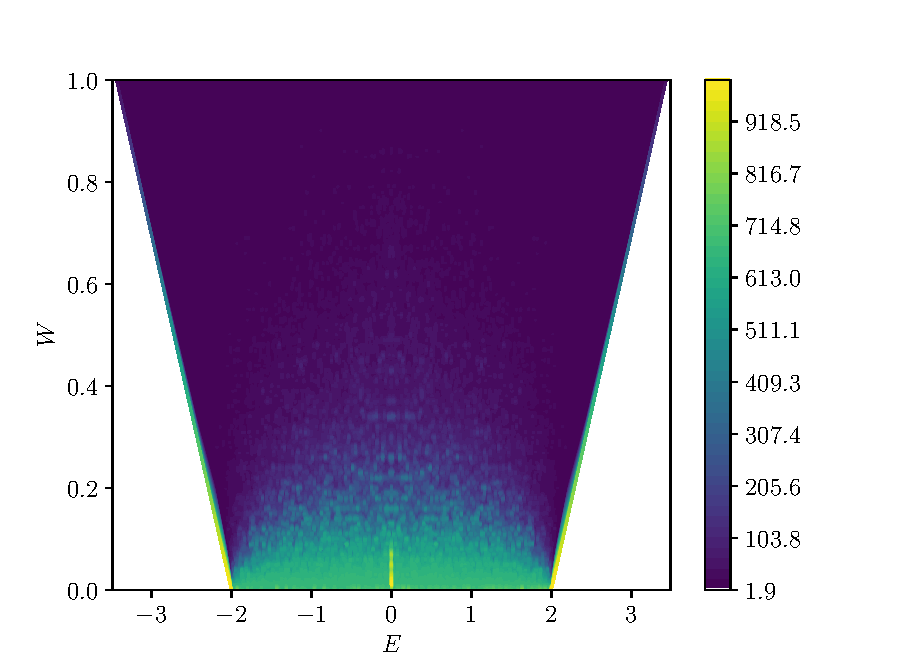
\includegraphics[width=\linewidth]{Figures/SSHIPR2.pdf}
\end{subfigure}
\caption{IPR za primer, ko je nered v sklopitvah. Na $x$ osi je energija stanj, na $y$ pa moč nereda $W$. Z barvo je označen IPR. Graf je pridobljen iz verige z dolžino 1000 mest.}
\label{fig:SSHIPR}
\end{figure}
V nadaljevanju bomo obranavali izključno primere, ko imamo nered na sklopitvah brez potencialov na posameznih mestih. Poglejmo si teorijo takšnih sistemov podrobneje.
Obravnavamo Hamiltonjan:
\begin{equation}
\hat{H} = \sum_i g_i \hat{c}_i^\dagger \hat{c}_{i+1} + \textup{h. c.},
\end{equation}
kjer so sklopitve $g_i$ neodvisne, enako porazdeljene naključne spremenljivke.
Pokazali bomo, da v tem primeru gostota stanj v okolici energije $E=0$ divergira kot:
\begin{equation}
g(E) \propto \frac{1}{E \log^3 E}
\end{equation}
Rešitev Schrödingerjeve enačbe z zgornjim Hamiltonjanom nastavimo kot:
\begin{equation}
| \Psi \rangle = \sum_i a_i  | i \rangle,
\end{equation}
kjer $|i \rangle$ predstavlja stanje, ki je lokalizirano na i-tem mestu verige.
Schrödingerjeva enačba se glasi:
\begin{equation}
a_{i-1} g_{i-1} + a_{i+1} g_i = E a_i,
\end{equation}
Vpeljimo količino $\Delta_i = a_{i-1} g_{i-1} / a_i$, ki po Schrödingerjevi enačbi zadošča $\Delta_{i+1} = g_i^2 / (E- \Delta_i)$. Označimo z $N(E)$ število stanj, z energijo, ki je manjša od $E$. Izkaže se \cite{dokazgostota}, da je to enako deležu pozitivnih $\Delta_i$. Iz rekurzivne formule za $\Delta_i$ vidimo, da pri $E=0$ ti po predznaku alternirajo, kar pomeni, da velja $N(0) = 0.5$.
Poglejmo si pozitivne $\Delta_i$. Brez izgube splošnosti lahko rečemo, da bodo ti sodi $\Delta_{2i}$.
Iz rekurzivne zveze sledi $\Delta_{2i} = (g_{2i-1}/g_{2i-2})^2 \Delta_{2i-2}$.
Če definiramo $u_{2i} = \ln \Delta_{2i}$, se ta zveza prevede v $u_{2i} = \ln (g_{2i-1}/g_{2i-2})^2 + u_{2i-2}$.
$u_{2i}$ torej opravljajo naključni sprehod v eni dimenziji za katerega velja:
\begin{align}
&\langle u_{2i} - u_{2i-2} \rangle = \langle \ln (g_{2i-1}/g_{2i-2})^2 \rangle = 2 \langle \ln g \rangle - 2 \langle \ln g \rangle = 0, \\
&\sigma_u^2 = \langle (u_{2i} - u_{2i-2})^2 \rangle = \langle (\ln (g_{2i-1}/g_{2i-2})^2)^2 \rangle = 2 \langle (\ln g^2)^2 \rangle - 2 \langle \ln g^2 \rangle^2 = 2 \sigma^2. 
\end{align}
V zadnji enačbi smo z $\sigma^2$ označili varianco $\ln g^2$.
Vemo, da naključni sprehodi ustrezajo difuzijskim procesom \cite{diffusion}, kjer za difuzijsko konstanto $D$ velja zveza $\sigma_u^2(t) = 2Dt$. V zgornji enačbi ima indeks $i$ vlogo časa, torej imamo $D=\sigma^2 / 2$. Označimo z $\phi (n, u)$ verjetnostno gostoto za $u_n$, ki mora zadoščati difuzijski enačbi:
\begin{equation}
2 \frac{\partial \phi (n,u)}{\partial n} = \sigma^2 \frac{\partial^2 \phi (n,u)}{\partial u^2}.
\end{equation}
Poglejmo si še primer, ko energija $E$ ni nič, vendar vseeno majhna.
Zaradi kiralne simetrije, se lahko omejimo na primer, ko velja $E > 0$.
Rekurzivna enačba za sode člene $\Delta_{2i}$ pri neničelni energiji je
\begin{equation}
\Delta_{2i} = \left(\frac{g_{2i -1}}{g_{2i-2}} \right)^2 \Delta_{2i-2} \frac{1 - E/\Delta_{2i-2}}{1+ (E \Delta_{2i-2} - E^2)/g_{2i-2}^2}
\end{equation}
V primeru, ko velja $E \ll \Delta_{2i-2} \ll g_{2i-2}^2/E$, so popravki k primeru $E=0$ zanemarljivi. $u$ torej še vedno opravlja naključni sprehod, dokler velja
$\ln E \ll u \ll \ln (g^2 / E)$, kjer je $g$ tu neka tipična vrednost sklopitve $g_i$, za katero se bo izkazalo, da ni pomembna. 
Ker imamo torej tudi pri neničelnem $E$ naključni sprehod, lahko tudi ta primer opišemo s prejšnjo difuzijsko enačbo. Poglejmo, kaj se zgodi z $u$, ko se približujemo zgornji in spodnji meji $\ln E$ in $\ln (g^2 / E)$, kar nam bo dalo robne pogoje za difuzijsko enačbo.
Pri zgornji meji $\Delta_{2i-2} \sim g^2/E$, imenovalec naraste, kar spet zmanjša $\Delta_{2i}$. Za naključni sprehod $u$ to pomeni, da imamo
odbijajočo bariero pri $u_{\textup{max}} = \ln (g^2 / E)$.
Pri spodnji meji, ko $\Delta_{2i-2} \sim E$ členi $\Delta_{2i}$ padajo, ko so enkrat pod $E$, pa se zgodi, da velja 
$\Delta_{2i+1} = g_{2i} / (E - \Delta_{2i}) > 0$. Eden izmed lihih členov, ki so do sedaj bili negativni torej spremeni predznak. Od tu naprej se zgodba ponavalja, členi spet alternirajo po predznaku, vendar so zdaj lihi tisti, ki so pozitivni, sodi pa negativni.
Zdaj imamo torej naslednjo sliko razvoja členov $\Delta_i$: Začnemo pri vrednosti $g^2/E$, nekaj časa padamo (ker smo na začetku pri odbijajoči barieri) in se začnemo naključno sprehajati.
Ko enkrat pridemo približno na vrednost $E$, se absorbiramo. Po tem se cikel ponovi, le da se vloge lihih in sodih zamenjajo.
Lahko vidimo, da potrebujemo dva cikla, da se eden izmed negativnih členov v alternirajočem zaporedju pri $E=0$ spremeni v pozitivnega. ZAKAJ DVA A SE NE PO ENEM? Torej, če rečemo, da je $\bar{n}$ povprečno število potrebnih korakov, po katerih se konča en cikel, imamo naslednjo relacijo za število stanj pod $E$:
\begin{equation}
N(E) - N(0) = N(E) - 0.5 = 1/(2\bar{n})
\end{equation}
Število $\bar{n}$ lahko dobimo na naslednji način.
Difuzijsko enačbo za $\phi$ opremimo z robnimi pogoji, katere smo izpeljali (bariera pri $u_{\textup{max}}$ in absorbcija pri $u_{\textup{min}}$)
\begin{align}
& \frac{\partial \phi}{\partial u} \vert_{u = u_{\textup{max}}} = 0 \\
& \phi \vert_{u = u_{\textup{min}}} = 0
\end{align}
Z začetnim pogojem $\phi (u, 0) = \delta ( u - u_{\textup{max}} - \epsilon)$.
Ko difuzijsko enačbo rešimo (na primer s seperacijo spremenljivk), lahko izračunamo:
\begin{equation}
P(n) = \int_{u_{\textup{min}}}^{u_{\textup{max}}} \phi(u,n) \textup{d} u,
\end{equation}
ki je verjetnost,da $u$ ostane med $u_{min}$ in $u_{max}$ (torej se ne absorbira) po n korakih.
Povprečno število korakov za en cikel je potem:
\begin{equation}
\bar{n} = \int_0^\infty n \left( - \frac{ \textup{d} P}{\textup{d} n} \right) \textup{d} n = \int_0^\infty P(n) \textup{d} n,
\end{equation}
kjer smo pri prvem enačaju uporabili definicijo pričakovane vrednosti v drugem pa integrirali per partes (robni členi so nič, saj seveda velja $P(\infty) = 0$).
Rešitev je $n =  \ln^2(g^2/E^2) / \sigma^2$ torej:
\begin{equation}
N(E) = 0.5 (1 + \sigma^2 / (\ln (g/E)^2)^2
\end{equation}
Kar pomeni, da je gostota stanj
\begin{equation}
g(E) = \frac{\textup{d} N}{\textup{d} E} = \frac{2 \sigma^2}{E} \frac{1}{\ln^3 (g/E)^2} = \frac{2 \sigma^2}{E |\ln E^2|^3},
\end{equation}
kjer smo lahko $g$ izpustili, saj predstavlja le (končno) aditivno konstantno divergirajočem imenovalcu.

\chapter{Model in metode dela}
Model, ki ga v tem delu obravnavamo, je nekoliko modificiran SSH model, opisan z naslednjim Hamiltonjanom:
\begin{equation}
\hat{H} = \sum_{n \in \mathbb{Z}} t_n \left( \frac{1}{2} \hat{c}_n^\dagger (\sigma_1 + i \sigma_2) \hat{c}_{n+1} + \textup{h.c.} \right) + m_n \hat{c}_n^\dagger \sigma_2 \hat{c}_n.
\end{equation}
Zaradi podobnosti z ostalimi deli na to temo \cite{mondragon} je notacija v tem razdelku drugačna kot v prej obdelanem SSH modelu, vendar lahko vseeno vidimo podobnosti: $t_n$ tukaj ustreza sklopitvi med različnimi osnovnimi celicami (prej $w$), medtem ko sklopitvi v osnovni celici (prej $v$) ustreza $\pm i m_n$. Ta model ni čisto enak kot SSH model, ker je ena izmed sklopitev imaginarna. S $c_n$ je označen vektor fermionskih operatorjev na obeh podmrežah, torej
$\hat{c}_n = (\hat{c}_{n,A} , \hat{c}_{n,B})^T$.
Model ima kiralno simetrijo \cite{mondragon}, kjer je operator kiralne simetrije enak:
\begin{equation}
\hat{S} = \sum_{n  \in \mathbb{Z}} \hat{c}_n^\dagger \sigma_3 \hat{c}_n.
\end{equation}
Nered bomo realizirali s pomočjo dveh naključno porazdeljenih spremenljivk - $\omega_n$ in $\omega_n^\prime$. Ti sta neodvisni in porazdeljeni po enakomerni porazdelitvi v intervalu $[ -0.5 , 0.5]$:
\begin{equation}
\omega_n, \omega_n^\prime \sim \mathcal{U}(-0.5,0.5).
\end{equation}
S temi nakjučnimi števili definiramo sklopitve na naslednji način:
\begin{align} \label{sklopitvi}
&t_n = 1 + 0.5 W \omega_n, \\
&m_n = m + W \omega_n^\prime.
\end{align}
Nered je torej centriran okoli vrednosti $1$ oziroma $m$, njegovo jakost pa podaja število $W$.
Če nered ni prisoten, imamo kot v SSH modelu na voljo dve topološki fazi, ki se ločita po ovojnem številu: $\nu=1$, če $m \in (-1,1)$ in $\nu=0$ sicer.

Ureditveni parameter v prisotnosti nereda bo še vedno ovojno število, vendar je njegov izračun tokrat nekoliko bolj zakompliciran.
Spomnimo se, da smo imeli v čistem sistemu na voljo formulo:
\begin{equation}
\nu = \frac{1}{2 \pi i} \int_0^{2 \pi} \frac{\partial \log h(k)}{\partial k} \textup{d}k = \frac{1}{2 \pi i} \int_0^{2 \pi} \frac{\partial h(k)}{\partial k} \frac{1}{h(k)} \textup{d}k,
\end{equation}
kjer je $h(k)$ naddiagonalna komponenta Hamiltonjana v recipročnem prostoru. V prisotnosti nereda nimamo več translacijske invariance in torej tudi nimamo več dobro določenega kristalnega valovnega vektorja. Očitno izraz za ovojno število v recipročnem prostoru ne bo dober, zato bomo zgornjo formulo zapisali v realnem prostoru.
To storimo z naslednjima substitucijama:
\begin{align}
&\frac{1}{2 \pi} \int_0^{2 \pi}\  \textup{d}k \to \frac{1}{N} \mathrm{Tr}, \\
&\frac{\partial}{\partial k} \to  -i [\hat{X}, \cdot ]. 
\end{align}
Prva formula predstavlja le zapis sledi na enoto volumna v drugi bazi. Drugo formulo lahko izpeljemo na naslednji način: 
Spomnimo se, da se v impulzni sliki operator kraja izraža kot $X = i \frac{\partial}{\partial k}$ (če postavimo $\hbar = 1$). Potem lahko takoj izračunamo:
\begin{equation}
 -i [\hat{X}, f(k)] \psi(k) =  \frac{\partial \left(f(k) \psi(k) \right)}{\partial k} - f(k) \frac{\partial \psi(k)}{\partial k} = \frac{\partial f(k)}{\partial k} \psi(k),
\end{equation}
s čimer smo pokazali želeno zvezo.


Pred spremembo baze smo imeli v integrandu izvendiagonalno komponento $h(k)$ Hamiltonjana v recipročnem prostoru. V realni bazi bo to sedaj $\frac{N}{2} \times \frac{N}{2}$ matrika: izvendiagonalni blok celotnega Hamiltonjana. Lažje bo računati s homotopsko ekvivalentnim Hamiltonjanom (spomnimo se, da homotopije ohranjajo ovojno število) $\hat{Q} = \hat{P}_+ -  \hat{P}_-$, kjer sta $\hat{P}_\pm$ projektorja na pozitivni oziroma negativni del spektra Hamiltonjana $\hat{H}$. Sedaj se spomnimo, da za operator kiralne simetrije $\hat{S}$ velja $\hat{S}^\dagger = \hat{S} $ in $\hat{S}^2 = \hat{\mathbb{I}}$, kar pomeni, da so njegove lastne vrednosti enake $\pm 1$. Zato ga lahko zapišemo kot $\hat{S} = \hat{S}_+ - \hat{S}_-$, kjer so $\hat{S}_\pm$ primerni sprektralni projektorji. Ker ima tudi Hamiltonjan $\hat{Q}$ kiralno simetrijo, ga lahko zapišemo kot
\begin{equation}
\hat{Q} = \hat{S}_+ \hat{Q} \hat{S}_- + \hat{S}_- \hat{Q} \hat{S}_+ = \hat{Q}_{+-} + \hat{Q}_{-+}.
\end{equation} 
Izvendiagonalni blok Hamiltonjana je potem preprosto $\hat{Q}_{+-}$, njegov inverz pa $\hat{Q}_{+-}^{-1} = \hat{Q}_{-+}$.
Sledi, da se formula za ovojno število glasi:
\begin{equation}
\nu = -\frac{1}{N} \mathrm{Tr} \left( \hat{Q}_{-+} [\hat{X},\hat{Q}_{+-}] \right).
\end{equation}
Zgornja formula velja, če računamo ovojno število za končno verigo brez robnih pogojev. Če pa želimo izračunati ovojno število za sistem s periodičnimi robnimi pogoji, (kot jo bomo v nadaljevanju), se moramo v zgornji formuli rešiti operatorja $\hat{X}$, kajti  pri sistemih s takimi robnimi pogoji je ta slabo definiran.
V tem primeru izrazimo namesto substitucije $\partial_k \hat{Q}_{+-} \to -i [\hat{X}, \hat{Q}_{+-}]$ odvod po $k$ s končnimi diferencami \cite{diference}:
\begin{equation}
\partial_k \hat{Q}_{+-}(k) = \sum_m c_m \hat{Q}_{+-} (k+m \Delta ), 
\end{equation}
kjer je najmanjša možna diferenca valovnega vektorja enaka $\Delta  = \frac{4 \pi}{N}$, saj ima naš sistem $N/2$ osnovnih celic.
Odvisnosti od $k$ v operatorju $\hat{Q}_{+-}$ se lahko znebimo s pomočjo operatorja $e^{i k \hat{x}}$, ki predstavlja translacijo za moment $k$: 
\begin{equation}
\hat{Q}_{+-}(k+m \Delta ) =e ^{-i m \Delta  \hat{x}} \hat{Q}_{+-}(k) e^{i m \Delta  \hat{x}}.
\end{equation}
Kot prej dobimo potem po prehodu v realni prostor formulo:
\begin{equation}
\nu = \frac{1}{N} \mathrm{Tr} (\sum_m c_m \hat{Q}_{-+} e^{-im \Delta \hat{x}} \hat{Q}_{+-} e^{im \Delta \hat{x}}).
\end{equation}
V zgornji formuli ni več težav z operatorjem $\hat{X}$, saj kompleksen eksponent poskrbi za periodičnost.
Iz formule za ovojno število brez periodičnih robnih pogojev je razvidno, da je v limiti močnega nereda $W \to \infty$ ovojno število enako nič, saj v tem primeru vezi v osnovni celici dominirajo in je komutator v formuli enak nič ($X$ označuje indeks osnovnih celic, ki so v tej limiti med sabo nesklopljene), medtem ko imamo po drugi strani pri $W=0$ in $m \in (-1,1)$ ovojno število enako ena. Ugotovili smo torej, da lahko med topološkimi fazami prehajamo tudi izključno z večanjem jakosti nereda. Tak prehod je prikazan na sliki \ref{fig:InvariantVsW}, na kateri se vidi, da ovojno število pri točki faznega prehoda $W=4$ praktično takoj pade z $1$ na $0$. Na sliki je tudi oblika energijskih pasov (valenčnega in prevodnega), kjer vidimo, da se ovojno število spremeni šele po tem, ko se energijska reža zapre, kar se zgodi že pri $W=3$.
\begin{figure}[H]
\centering
\begin{subfigure}{.7\textwidth}
\includegraphics[width=\linewidth]{Figures/InvariantVsW.png}
\end{subfigure}
\caption{ovojno število v odvisnosti od jakosti nereda pri $m=0$, kjer so rezultati povprečeni po $200$ realizacijah nereda. Opazimo nenadno spremembo pri približno $W=4$, medtem ko se energijska reža zapre pri $W=3$. Vir slike: \cite{mondragon}}
\label{fig:InvariantVsW}
\end{figure}

Izkaže se, da točke faznega prehoda sovpadajo s točkami divergence lokalizacijske dolžine stanja z ničelno energijo. Zaradi Andersonove lokalizacije so stanja v prisotnosti nereda lokalizirana, a pride pri faznem prehodu do tranzicije v delokalizirano stanje pri energiji nič.
To se da videti iz eksplicitne rešitve Schrödingerjeve enačbe pri energiji nič. Označimo to rešitev z $|  \Psi \rangle$.
To stanje lahko zapišemo kot:
\begin{equation}
| \Psi \rangle = \sum_{\substack{n \in \mathbb{Z} \\ \alpha \in \{-1,1\}}} \Psi_{n, \alpha} |n, \alpha \rangle,
\end{equation}
kjer $n$ označuje indeks osnovne celice, $\alpha=1$ ustreza podmreži A, $\alpha=-1$ pa podmreži B.
Schrödingerjeva enačba se glasi:
\begin{align}
&H \Psi = 0, \\
&t_n \psi_{n-\alpha, \alpha} + i \alpha m_n \Psi_{n, \alpha} = 0.
\end{align}
Iz zgornje enačbe lahko rekurzivno izrazimo rešitev:
\begin{equation}
\Psi_{n+\xi_\alpha, \alpha} = i^n \prod_{j=1}^n \left( \frac{t_j}{m_j} \right)^\alpha \Psi_{\xi_\alpha,\alpha},
\end{equation}
kjer $\alpha = \pm 1$ ustreza $\xi_\alpha = 0, 1$.
Za velike $n$ definirajmo $|\Psi_{n+\xi_\alpha, \alpha}| = e^{-n/\Lambda } |\Psi_{\xi_\alpha, \alpha}|$, saj mora valovna funkcija eksponentno padati, če hočemo, da je normalizabilna. Z $\Lambda$ smo označili lokalizacijsko dolžino stanja.
Iz zgornje rekurzivne enačbe dobimo izraz zanjo:
\begin{equation}
\Lambda^{-1} = \left| - \lim_{n \to \infty} \frac{1}{n} \log |\Psi_{n+ \xi_\alpha, \alpha}| / |\Psi_{\xi_\alpha, \alpha}| \right|.
\end{equation}
Izkaže se, da je izraz na desni neodvisen od izbire podmreže $\alpha$ (zgodi se le, da izraz znotraj absolutne vrednosti spremeni predznak).
Če vstavimo rekurzivni izraz za $\Psi_{n+ \xi_\alpha, \alpha}$, dobimo:
\begin{equation} \label{empiricnalok}
\Lambda^{-1} = \left| \lim_{n \to \infty} \frac{1}{n} \sum_{j=1}^n ( \log |t_j| - \log |m_j| ) \right| 
\end{equation}
Zgornjo formulo bi radi poenostavili. 
To lahko naredimo s pomočjo Birkhoffovega ergodičnega izreka \cite{birkhoff}:
\begin{theorem*}
Naj bo $X$ stacionaren in ergodičen stohastični proces in $f$ takšna funkcija, da velja $E(|f|) < \infty$. Potem velja:
\begin{equation}
\lim_{n \to \infty} \frac{1}{n} \sum_{j=1}^{n} f(\theta_j x) = E(f),
\end{equation}
kjer je $\theta_j (x_1,x_2,x_3, \dots) = (x_2,x_3,x_4, \dots)$ operator premika, $E(f)$ pa označuje pričakovano vrednost $f$.
\end{theorem*}
V našem primeru predstavlja stohastični proces $X$ vzorce naših naključnih spremenljivk $X=((t_1,m_1),(t_2,m_2),(t_3,m_3), \dots)$. Ta proces je stacionaren in ergodičen, saj so posamezni vzorci neodvisni in enako porazdeljeni \cite{birkhoff} (teorem sicer velja tudi v splošnejših primerih, ko so vzorci na primer paroma korelirani).
Funkcija $f$ je v našem primeru enaka  $f((x_1,y_1),( x_2, y_2), ...) = \log |x_1| - \log |y_1|$.
Poglejmo si pričakovano vrednost $|f|$:
\begin{equation}
E(|f|) = \int_{-0.5}^{0.5} \textup{d} \omega \int_{-0.5}^{0.5} \textup{d} \omega^\prime \left| \log | 1 + W_1 \omega | - \log | m + W_2 \omega^\prime | \right|.
\end{equation}
Ker integriramo po končnem intervalu, je morebiten problematičen del le tisti, kjer ima logaritem divergenco, na primer, ko velja $\omega \sim -\frac{1}{W_1}$. Ko primerno razbijemo integral na manjše intervale in se znebimo absolutne vrednosti v integrandu, dobi tak problematičen del obliko $\lim_{\epsilon \to 0} \int_{- \epsilon}^\epsilon \log |x| dx =  2 \lim_{\epsilon \to 0} \int_{0}^\epsilon \log x dx = \lim_{\epsilon \to 0} x (\log x - 1) \rvert_0^\epsilon = 0$. Del blizu divergence torej k intergalu ne prispeva in velja $E(|f|) < \infty$.

Sedaj lahko direktno uporabimo Birkhoffov izrek, da dobimo:
\begin{equation}
\Lambda^{-1} = \left| \int_{-0.5}^{0.5} \textup{d} \omega \int_{-0.5}^{0.5} \textup{d} \omega^\prime ( \log | 1 + W_1 \omega | - \log | m + W_2 \omega^\prime | ) \right|,
\end{equation}
kar se da analitično izračunati. Rezultat je:
\begin{equation} \label{analiticnalok}
\Lambda^{-1} = \left| \log( \frac{|2+W_1|^{1/W_1 + 0.5} |2m - W_2|^{m/W_2 -0.5}}{|2-W_1|^{1/W_1-0.5} |2m + W_2|^{m/W_2 + 0.5}})\right|.
\end{equation}

\begin{figure}[H]
\centering
\begin{subfigure}{.7\textwidth}
\includegraphics[width=\linewidth]{Figures/CriticalSurface.png}
\end{subfigure}
\caption{na levi je prikazan fazni diagram modela. Na desni je prikazana še lokalizacijska dolžina stanja z $E=0$, ki divergira vzdolž faznega prehoda in je enaka $0$ zunaj tega območja. Prav tako je na desni z zeleno črto označena pot, po kateri bomo pozneje izvedli preklop Hamiltonjana. Izračuni za $\nu$ so narejeni na verigi velikosti $N=2000$ in povprečeni preko $10$ realizacij nereda. Vir slike: \cite{mondragon}}
\label{fig:CriticalSurface}
\end{figure}

Na sliki \ref{fig:CriticalSurface} je prikazan fazni diagram našega modela. Opazimo, da divergenca lokalizacijske dolžine pri ničelni energiji res sovpada s točkami faznega prehoda. Kot prej povedano, lahko poleg prehajanja med fazama, ki smo ga videli že v SSH modelu, preidemo med fazama tudi z dovolj močno jakostjo nereda. Zanimali nas bodo preklopi Hamiltonjana čez fazni prehod, kjer bomo povečevali $W$ pri $m=0$, kot je na desnem grafu označeno z zeleno črto.
Zaenkrat nekaj o tem faznem prehodu že vemo: Če razvijemo enačbo (\ref{analiticnalok}) okoli $W_C=4$, pri $m=0$, vidimo, da lokalizacijska dolžina v bližini faznega prehoda skalira kot $\Lambda \sim \frac{1}{|W-W_C| \log |W-W_C|}$. Kritični eksponent $\nu$ za ta prehod je torej enak ena z logaritemskim popravkom.

Oglejmo si obnašanje modela vzdolž poti, preko katere bomo izvedli preklop. 
Kot prvi test in občutek za potrebno velikost verige $N$, si poglejmo primerjavo empirične (\ref{empiricnalok}) in analitične (\ref{analiticnalok}) formule za lokalizacijsko dolžino vzdolž te poti za več velikosti sistema.
\begin{figure}[H]
\centering
\begin{subfigure}{\textwidth}
\includegraphics[width=\linewidth]{Figures/locLength.pdf}
\end{subfigure}
\caption{inverz lokalizacijske dolžine, pridobljen z empirično formulo za več velikosti sistema ($N$ prikazuje število vseh atomov v verigi) in z analitično formulo za neskončno dolgo verigo vzdolž poti $W: 2 \to 6$ pri $m=0$.}
\label{fig:locLength}
\end{figure}
Na sliki \ref{fig:locLength} vidimo, da za velikosti verige nekaj tisoč atomov še ne pridemo do točnega asimptotskega obnašanja - za to potrebujemo verigo dolžine več sto tisoč atomov - , vendar je obnašanje lokalizacijske dolžine pri tako majhnih verigah vseeno kvalitativno zelo podobno obnašanju neskončne verige. Za večje $N$ postane numerika zelo zahtevna, zato bom v nadaljevanju (če ne bo drugače rečeno) obravnaval verigo z $N=1000$. Vse izračune, ki sledijo, sem ponovil za dvakrat daljšo verigo, kjer ni bilo opaziti bistvenih razlik. Poleg tega lahko na sliki opazimo še naslednje: ko imamo opravka z določeno realizacijo nereda, je število uporabljenih naključnih števil seveda končno in se divergenca lokalizacijske dolžine (in s tem fazni prehod) ne zgodi točno pri $W=4$, kot narekuje asimptotska formula, temveč v bližini te točke. Izkaže se, da to ni problem, saj bomo pri eksitacijah rezultate tako ali tako povprečevali po dovolj veliko realizacijah nereda, da lahko privzamemo, da je povprečna točka faznega prehoda res $W=4$.

Sedaj si poglejmo, kako izgledajo energijski nivoji vzdolž prej omenjene poti čez fazni prehod. 
V ta namen napišimo Hamiltonjan v matrični obliki:
\[
H = \begin{bmatrix} 
0 & i m_1 &  &  &  & t_{N/2}\\
-i m_1 & 0 & t_1 &  & &  \\
 & t_1 & 0 & im_2 &  &  \\
 &  & -im_2 & 0& \ddots&  & \\
 &  &  & \ddots & \ddots & im_{N/2}  \\
t_{N/2} & & &  & -i m_{N/2} & 0  
    \end{bmatrix}
\]
Izbrali smo periodične robne pogoje, saj se hočemo čim bolj približati neskončni verigi. Energije bomo dobili z diagonalizacijo zgornje matrike.
Iz spektra lahko izračunamo tudi gostoto stanj. Formalno je to vsota Diracovih delta funkcij pri lastnih energijah:
\begin{equation}
g(E) = \sum_{i=1}^N \delta (E_i - E).
\end{equation}
Za potrebe prikaza bom Diracove delte aproksimiral z Lorentzovo krivuljo:
\begin{equation}
\delta (x) = \lim_{\sigma \to 0} \frac{1}{\pi} \frac{\sigma}{\sigma^2 + x^2}.
\end{equation}
V mojih izračunih sem vzel vrednost $\sigma=0.01$.
Rezultati, ki jih da numerika, so sledeči:
\begin{figure}[H]
\centering
\begin{subfigure}{\textwidth}
\includegraphics[width=\linewidth]{Figures/Nicegraph.pdf}
\end{subfigure}
\caption{na zgornjem grafu je prikazanih nekaj najnižjih lastnih energijskih nivojev vzdolž poti $W: 2 \to 6$ pri $m=0$. S črno črtkano črto (desna y os) je narisana lokalizacijska dolžina za to realizacijo nereda. Na spodnjih treh grafih je za različna mesta vzdolž poti prikazana gostota stanj.}
\label{fig:Nicegraph}
\end{figure}
Na sliki \ref{fig:Nicegraph} vidimo nekaj najnižjih pozitivnih energijskih nivojev vzdolž poti, kjer bomo izvajali preklop. Slika za negativne je enaka, saj je zaradi kiralne simetrije spekter simetričen. Vidimo, da se pri približevanju kritični točki energijska reža res zapira. S primerjanjem gostot stanj pri večjih velikostih sistema smo potrdili, da se reža zapre pri $W=3$. Podrobnejše obnašanje energijskih nivojev je precej naključno, po prehodu skozi kritično točko pa se energijska reža odpira veliko počasneje in je v praksi kar še vedno zaprta. Opazimo, da se energijski nivoji med seboj večkrat sekajo, pogosto pa pride tudi do odboja nivojev, kot je na primer prikazano na povečanem delu grafa.
Na grafu je prikazana tudi lokalizacijska dolžina stanja z energijo nič in vidimo lahko, da se v točki, kjer ta divergira, energijski nivoji res najbolj približajo ničli, kar ustreza faznemu prehodu med topološkima fazama. V resnici gredo čisto na nič, vendar smo tu seveda omejeni z numeriko in torej končnim sistemom. 
Na spodnjih treh grafih je prikazana gostota stanj, pridobljena za tri točke vzdolž poti. Prva ustreza $W=2$, kar je še daleč od kritične točke, kjer je energijska reža še odprta, kar vidimo v ničelni gostoti stanj okoli energije nič. Okoli $W=3$ se energijska reža že zapira, kar lahko potrdimo s tem, da je gostota stanj pri $E=0$ že neničelna. V kritični točki se v gostoti stanj pojavi divergenca pri energiji $0$. Točno obliko te divergence pravzaprav že slutimo: če v formuli \ref{sklopitvi} za sklopitvi $t_n$ in $m_n$ vstavimo $W=4$, opazimo, da so velikosti obeh sklopitev porazdeljene po isti porazdelitvi. Obnašanje gostote stanj v primeru, ko so sklopitve enako porazdeljene pa poznamo in smo izpeljali v prejšnjem poglavju: $g(E) \propto \frac{1}{E \log^3 E}$.
Situacija pa ni čisto ista kot pri izpeljavi te formule, saj je ena izmed sklopitev imaginarna. Histogram na sliki \ref{fig:dos} prikazuje porazdelitev števila stanj po energijah pri $W=4$, pridobljen za sistem z $N=75000$ osnovnimi celicami z odprtimi robnimi pogoji. Število stanj v majhnem intervalu energije je sorazmerno povprečni gostoti stanj na sredini tega intervala, kar pomeni, da ima prikazani histogram isto obliko kot gostota stanj. Vidimo, da se prilagojena krivulja $g(E) \propto \frac{1}{E \log^3 E}$ s histogramom res ujema in da velja prej izpeljana formula za gostoto stanj tudi v našem primeru.

\begin{figure}[H]
\centering
\begin{subfigure}{.9\textwidth}
\includegraphics[width=\linewidth]{Figures/DOS.pdf}
\end{subfigure}
\caption{histogram lastnih energij za sistem velikosti $N=75000$ pri odprtih robnih pogojih.}
\label{fig:dos}
\end{figure}

Na sliki \ref{fig:SSHIPRNered} je prikazan IPR za model, ki ga obravnavamo. Tu so že v čistem modelu stanja lokalizirana, saj čisti model ustreza eni izmed popolnoma dimeriziranih limit v SSH modelu. Ko dodamo nered, ostanejo stanja močno lokalizirana. Tudi v okolici točke $W=4, E=0$ ni videti nobene delokalizacije, kar se zdi v nasprotju z našo prejšnjo izpeljavo. Razlog za to je dejstvo, da velja delokalizacija točno v kritični točki in točno pri energiji nič, kar sta pogoja, katerima lahko z numeriko zadostimo le do določene natančnosti in torej tega v praksi ne opazimo.

\begin{figure}[H]
\centering
\begin{subfigure}{.7\textwidth}
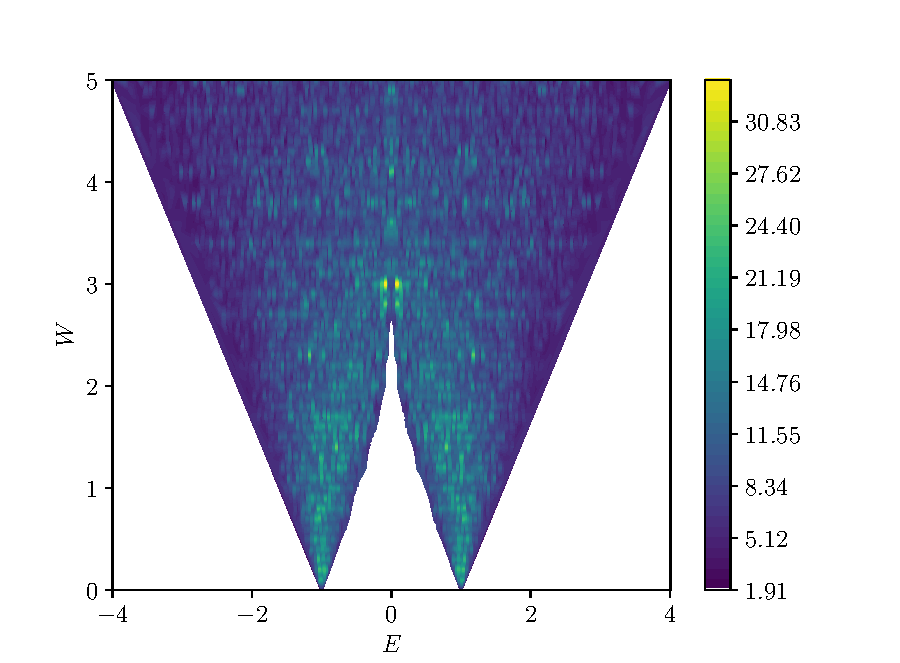
\includegraphics[width=\linewidth]{Figures/SSHIPRNered.pdf}
\end{subfigure}
\caption{IPR v odvisnosti od jakosti nereda $W$ in energije $E$.}
\label{fig:SSHIPRNered}
\end{figure}
Na sliki \ref{fig:EigenPloti} so prikazane nekatere lastne funkcije modela pred točko faznega prehoda in v njej. Opazimo, da so vse lokalizirane, čeprav se v kritični točki že vidi drugačno obnašanje stanja z najmanjšo energijo. To ima, za razliko od ostalih, posamezna vrhova precej daleč narazen. V termodinamski limiti postane prav to stanje delokalizirano, vendar ga v končnih sistemih kot na Sliki \ref{fig:SSHIPRNered} ne bomo našli. Stanje z najnižjo energijo na levem grafu slike posameznih vrhov nima zares daleč narazen, saj imamo opravka s periodičnimi robnimi pogoji.
\begin{figure}[H]
\centering
\begin{subfigure}{.7\textwidth}
\includegraphics[width=\linewidth]{Figures/EigenPloti.pdf}
\end{subfigure}
\caption{na levi so prikazane prve 3 lastne funkcije s pozitivno energijo pri $W=3.8$, na desni pa pri $W=4$.}
\label{fig:EigenPloti}
\end{figure}
Sedaj se bomo posvetili preklopom Hamiltonjana čez fazni prehod, kar pomeni, da bomo spremljali časovni razvoj valovne funkcije, pri čemer bomo parametre Hamiltonjana linearno spreminjali vzdolž prej omenjene poti.

Preklop delamo med dvema vrednostima jakosti nareda, tako da začnemo pri vrednosti $W_{\textup{z}}<4$, končamo pa, po določenem času preklopa $T$, pri vrednosti $W_{\textup{k}}>4$.
Časovno odvisnost jakosti nereda lahko torej zapišemo kot: 
\begin{equation}
W(t) = W_{\textup{zac}} +  t/T (W_{\textup{konc}}-W_{\textup{zac}}).
\end{equation} 
Začnemo v lastnem stanjem iz valenčnega pasu pri $W_{\textup{z}}$ in ga časovno razvijemo. Ker delamo preklop, je tudi Hamiltonjan odvisen od časa.
Rešujemo torej časovno odvisno Schrödingerjevo enačbo:
\begin{equation}
i \frac{\partial \Psi}{\partial t} = \hat{H}(t) \Psi.
\end{equation}
Rešitev izrazimo s pomočjo operatorja časovnega razvoja $\hat{U}(t) = e^{-i \hat{H}(t) t}$ kot $\Psi(t+\tau) \approx \hat{U}(t) \Psi(t)$.
Za numeričen izračun časovnega razvoja bomo uporabili implicitno metodo tipa Crank-Nicholson, ki zagotavlja, da je operator časovnega razvoja unitaren.
Uporabili bomo Padéjevo aproksimacijo za eksponentno funkcijo:
\begin{equation}
\exp (-i \tau \hat{H}) = \left(\hat{\mathbb{I}} + i \frac{\tau}{2} \hat{H} \right)^{-1}   \left(\hat{\mathbb{I}} - i \frac{\tau}{2} \hat{H} \right) + \mathcal{O}(\tau^3),
\end{equation} 
s čimer dobimo implicitno shemo:
\begin{equation}
\left( \hat{\mathbb{I}} + i \frac{\tau}{2} \hat{H}(t) \right) \Psi (t+\tau) = \left(\hat{\mathbb{I}}- i \frac{\tau}{2} \hat{H}(t) \right) \Psi(t).
\end{equation}
V našem primeru bomo časovno razvijali več funkcij hkrati. To bi lahko storili tako, da bi zgornjo enačbo reševali za vsako izmed njih, a je učinkoviteje, če rešujemo matrično enačbo:
\begin{equation}
\left( \mathbb{I} + i \frac{\tau}{2} \hat{H}(t) \right) X(t+\tau) = \left(\mathbb{I}- i \frac{\tau}{2} \hat{H}(t) \right) X,
\end{equation}
kjer so v matriki $X$ lastni vektorji $\Psi$ v stolpcih.
V našem primeru bomo vzeli vrednost $\tau=1$. Rezultate smo preverili tudi pri $\tau=0.5$, kjer nismo opazili nobene razlike.

Med preklopom se pojavijo eksitacije v prevodnem pasu, saj je čas preklopa končen.
Število eksitacij v i-to stanje oziroma zasedenost i-tega stanja izračunamo preprosto kot
\begin{equation}
N_i = \sum_j |\langle i | \Psi_j \rangle|^2,
\end{equation}
kjer je $\Psi_j$ časovno razvito j-to stanje iz valenčnega pasu, $| i \rangle$ pa predstavlja i-to lastno stanje Hamiltonjana ob nekem času. Vrednost $| \langle i | \Psi_j \rangle |^2$ je verjetnost, da preskoči elektron iz časovno razvitega stanja $\Psi_j$ v lastno stanje $| i \rangle$. Celotno verjetnost za prehod v stanje $| i \rangle$ in s tem zasedenost tega stanja potem dobimo tako, da to seštejemo po vseh časovno razvitih stanjih iz valenčnega pasu $\Psi_j$.

Pri obravnavi eksitacij bomo iskali odvisnosti oblike 
\begin{equation}
N_{\textup{eks}} = \alpha T^{\beta},
\end{equation}
pri čemer nas bo zanimala predvsem potenca $\beta$. Za natančno pridobitev le-te iz podatkov zgornjo enačbo najprej logaritmiramo
\begin{equation}
\log N_{\textup{eks}} = \log \alpha + \beta \log T.
\end{equation}
Z definicijami $y=\log N_{\textup{eks}}$ in $x=\log T$, tako dobimo linearno funkcijo $y=\beta x + \log \alpha$, ki jo lahko natančno prilagajamo podatkom.

\chapter{Rezultati preklapljanja}
Poglejmo, kolikšno je število eksitacij po preklopu za več različnih preklopov. Na levem grafu slike \ref{fig:Skaliranje} se vidi, da število eksitacij pada z dolžino preklopa, kar je smiselno, saj vemo, da adiabatski preklop ustreza neskončno dolgemu preklopu, v katerem se eksitacije ne pojavijo.
Prav tako opazimo, da imamo več eksitacij, če preklapljamo na večjem intervalu jakosti nereda $[W_{\textup{z}}, W_{\textup{k}}]$. To se zgodi, ker pri najmanjšem intervalu jakosti nereda preklopa ne začnemo dovolj globoko v topološki fazi in smo pravzaprav že na meji, kjer se energijska reža zapira, kot se bo pokazalo na sliki \ref{fig:SkoziCas}. Vidimo lahko tudi, da število eksitacij na območju počasnejših preklopov skalira kot potenčni zakon, kjer je potenca odvisna od intervala jakosti nereda, preko katerega delamo preklop. Potenčno funkcijo sem tu prilagodil na tri najpočasnejše preklope. Kot bo vidno na sliki \ref{fig:SkoziCas}, so hitrejši preklopi prehitri, kar povzroči, da imamo veliko eksitacij že takoj na začetku preklopa, podobno kot če preklapljamo po premajhnem intervalu jakosti nereda.
\begin{figure}[H]
\centering
\begin{subfigure}{.99\textwidth}
\includegraphics[width=\linewidth]{Figures/Skaliranje3Alt.pdf}
\end{subfigure}
\caption{na levi je prikazano število vseh eksitacij po koncu preklopa v odvisnosti od njegovega časa trajanja $T$, na desni pa v odvisnosti od njegove hitrosti $v$. S črtkanimi črtami je prikazana ekstrapolacija iz treh točk pri največjih časih $T$. Podatki so prikazani za 3 različne izbire $W_{\textup{z}}$ in $W_{\textup{k}}$.}
\label{fig:Skaliranje}
\end{figure}
Pravzaprav je smiselneje gledati število eksitacij v odvisnosti od hitrosti preklopa (namreč, preklop $3.5 \rightarrow 4.5$ pri $T=10000$ je enako hiter kot preklop $2 \rightarrow 6$ pri $T=40000$), kar je prikazano na desnem grafu slike \ref{fig:Skaliranje}. Tu jasneje opazimo, da sta si preklopa na daljšem intervalu veliko bolj podobna v obnašanju - v primerjavi s preklopom na krajšem intervalu. 
\begin{figure}[H]
\centering
\begin{subfigure}{.99\textwidth}
\includegraphics[width=\linewidth]{Figures/SkoziCas.pdf}
\end{subfigure}
\caption{skupno število eksitacij med preklopom, prikazano za več različnih intervalov preklopa in njihovih hitrosti.}
\label{fig:SkoziCas}
\end{figure}
Na sliki \ref{fig:SkoziCas} opazimo prej omenjeno hitro naraščanje števila eksitacij že takoj na začetku preklopa pri ozkem intervalu preklopa ter pri hitrih preklopih.
Pri daljših intervalih in počasnejših preklopih vidimo, da je krivulja na začetku vodoravna, kar pomeni, da smo začeli dovolj globoko, ko je energijska reža še dovolj široka, da eksitacij ni. Podobno kot v energijskih nivojih se pojavi asimetrija območja pred in po kritični točki $W=4$.
Na sliki \ref{fig:SkoziCasAlt} smo graf eksitacij skozi čas v x osi reskalirali s prej dobljenimi eksponenti za potenčno odvisnost števila eksitacij od dolžine preklopa, število eksitacij na koncu preklopa pa normirali na $1$. Opazimo univerzalno obnašanje krivulj pri preklopih na daljšem intervalu. Najhitrejši preklopi odstopajo iz tega obnašanja, vendar smo to pričakovali, saj smo že povedali, da spadajo ti v drugačen režim, kjer se veliko eksitacij pojavi že takoj na začetku preklopa.
\begin{figure}[H]
\centering
\begin{subfigure}{.99\textwidth}
\includegraphics[width=\linewidth]{Figures/SkoziCasAlt.pdf}
\end{subfigure}
\caption{skupno število eksitacij med preklopom, prikazano za več različnih intervalov preklopa in njihovih hitrosti, kjer je vsak graf reskaliran s primerno potenco, pridobljeno iz slike \ref{fig:Skaliranje}.}
\label{fig:SkoziCasAlt}
\end{figure}
Poglejmo si še, kje natančneje se pojavijo te eksitacije. Na sliki \ref{fig:Krajevne} je prikazana krajevna porazdelitev eksitacij med preklopom. Vidimo, da se eksitacije pojavijo na naključnih osnovnih celicah, katere zasedenost potem s časom še raste.
\begin{figure}[H]
\centering
\begin{subfigure}{.99\textwidth}
\includegraphics[width=\linewidth]{Figures/KrajevneEksitacijeNoGrid.pdf}
\end{subfigure}
\caption{na sliki so histogrami krajevne porazdelitve eksitacij po indeksih na verigi s $500$ osnovnimi celicami po koncu preklopa, ki traja $T=6000$ in poteka na intervalu $W=[3,5]$.}
\label{fig:Krajevne}
\end{figure}

Poglejmo si še porazdelitev eksitacij po lastnih stanjih Hamiltonjana ob nekih fiksnih časih. To je prikazano na sliki \ref{fig:EksTekom} za dve realizaciji nereda. Kot smo že videli, na začetku, ko je energijska reža še dovolj široka, še nimamo eksitacij. Nekje pri $W=4$ se eksitacije začenjajo pojavljati in ostanejo še po preklopu. 

\begin{figure}[H]
\centering
\begin{subfigure}{.49\textwidth}
\includegraphics[width=\linewidth]{Figures/EksTekom1.pdf}
\end{subfigure}
\begin{subfigure}{.49\textwidth}
\includegraphics[width=\linewidth]{Figures/EksTekom2.pdf}
\end{subfigure}
\caption{energijski nivoji in eksitacije za dve realizaciji nereda. Število eksitacij predstavljata velikost in barva pikic. Hitrost preklopa je $v=0.01$ na intervalu $W \in [3,5]$.}
\label{fig:EksTekom}
\end{figure}
Na sliki \ref{fig:EksBini} smo interval energij $E \in [10^{-13},10^{-4}]$ v logaritemski skali razdelili na 20 enako velikih območij in opazovali eksitacije, ki padejo vanje, povprečene preko $100$ realizacij nereda. Prikazana sta grafa za dve različni hitrosti preklopa. Ta grafa služita le kot nazornejša slika prej omenjenega dejstva, da je po kritični točki prisotnih veliko več eksitacij kot pred njo in da se začenjo pri hitrejšem preklopu eksitacije pojavljati že nekoliko preden se približamo kritični točki.
\begin{figure}[H]
\centering
\begin{subfigure}{.49\textwidth}
\includegraphics[width=\linewidth]{Figures/EksBini1.pdf}
\end{subfigure}
\begin{subfigure}{.49\textwidth}
\includegraphics[width=\linewidth]{Figures/EksBini2.pdf}
\end{subfigure}
\caption{eksitacije na interval energije med preklopom. Interval $E \in [10^{-13},10^{-4}]$ smo razdelil na 20 enako velikih delov v logaritemski skali in narisali povprečno število eksitacij za vsak interval, povprečeno po $100$ realizacijah nereda. Na levi je $v=0.001$ na desni pa $v=0.0001$.}
\label{fig:EksBini}
\end{figure}
Na sliki \ref{fig:EksBini2} vidimo podobna grafa, vendar tokrat za večji interval energije $E \in [10^{-13},1]$ in v logaritemski skali. Opazimo, da imajo po počasnejšem preklopu najvišje vzbujeni elektroni manjšo energijo, kot pri hitrejšem. Tudi to bi lahko pričakovali, saj že vemo, da imamo nasploh več eksitacij v hitrejših preklopih.
\begin{figure}[H]
\centering
\begin{subfigure}{.49\textwidth}
\includegraphics[width=\linewidth]{Figures/EksBini3.pdf}
\end{subfigure}
\begin{subfigure}{.49\textwidth}
\includegraphics[width=\linewidth]{Figures/EksBini4.pdf}
\end{subfigure}
\caption{eksitacije na interval energije med preklopom. Interval $E \in [10^{-13},1]$ smo razdeliil na 50 enako velikih delov v logaritemski skali in narisali povprečno število eksitacij za vsak interval, povprečeno po $100$ realizacijah nereda. Grafa sta tokrat v logaritemski skali. Leva $v=0.001$, desna $v=0.0001$.}
\label{fig:EksBini2}
\end{figure}

Na sliki \ref{fig:Emax} si podrobneje pogledamo, kako je z ravnokar omenjenim višanjem energij vzbujenih elektronov s hitrostjo preklopa. Opazujemo, pri kateri energiji pade zasedenost stanj z $0.5$ na $0.25$, kar služi kot ocena za robno energijo, nad katero ni več veliko eksitacij. Če to narišemo v odvisnosti od hitrosti preklopa, opazimo, da je odvisnost spet potenčna, vendar je eksponent občutljiv na finost particije intervala energije in se giblje okoli vrednosti $0.5$.
\begin{figure}[H]
\centering
\begin{subfigure}{\textwidth}
\includegraphics[width=\linewidth]{Figures/Emax.pdf}
\end{subfigure}
\caption{na grafu je prikazana energija najvišje zasedenih stanj po koncu preklopa za več njegovih hitrosti. To je energija, kjer eksitacije prvič padejo na $0.25$. Rezultati so povprečeni po $100$ realizacijah nereda, energijski interval pa je razdeljen na $500$ delov. Preklop je potekal na intervalu $W:\ 3 \to 5$.}
\label{fig:Emax}
\end{figure}
Na sliki \ref{fig:IzEngaStanja} lahko vidimo, kam točno prehaja elektron, ki je na začetku v nekem izbranem stanju. Na sliki je prikazano prvo stanje z negativno energijo, vendar je obnašanje podobno pri ostalih nizkoenergijskih stanjih. Opazimo, da preidemo po kritični točki z verjetnostjo približno $0.5$ v prevodni pas, v katerem imamo praviloma na voljo dve stanji, v kateri lahko preidemo z verjetnostjo $0.25$. Ti stanji, v kateri lahko skočimo, sta ravno kiralna partnerja stanj, v katerih ostanemo, če ne pride do skoka v prevodni pas.  
\begin{figure}[H]
\centering
\begin{subfigure}{\textwidth}
\includegraphics[width=\linewidth]{Figures/IzEngaStanja.pdf}
\end{subfigure}
\caption{na grafu je z barvo prikazana verjetnost za prehod v različna lastna stanja Hamiltonjana med preklopom, če preklapljamo lastno stanje, ki ima na začetku najvišjo negativno energijo (torej prvo stanje v valenčnem pasu) pri neki realizaciji nereda. Zgornji graf prikazuje prevodni pas, spodnji pa valenčnega. Na grafu so označena tudi zaporedna števila stanj, v katera prehajamo.}
\label{fig:IzEngaStanja}
\end{figure}
Opazili smo, da se po prehodu skozi točko faznega prehoda lahko indeksi zasedenih stanj še nadalje spreminjajo. Razlago za to lahko vidimo na sliki \ref{fig:IzEngaStanjaWBand}. Po prehodu ostanejo energijski nivoji tesno blizu in se pogosto križajo, kar povzroči , da se naše začetno stanje preimenuje v drugega. Poleg križanja se lahko pojavijo tudi odboji energijskih nivojev, pri katerih lahko elektron še nadalje skoči na naslednji energijski nivo.

\begin{figure}[H]
\centering
\begin{subfigure}{\textwidth}
\includegraphics[width=\linewidth]{Figures/IzEngaStanjaWBand.pdf}
\end{subfigure}
\caption{na grafu je nekaj najnižjih energijskih nivojev v prevodnem pasu. S pikicami so označene verjetnosti za prehod v prevodni pas, če preklapljamo stanje z najvišjo energijo v valenčnem pasu.}
\label{fig:IzEngaStanjaWBand}
\end{figure}

%\input{Zaklju"cek}
\chapter{Zaklju"cek}
Obravnavali smo prirejen SSH model z imaginarno sklopitvijo v osnovnih celicah. Model ustreza enodimenzionalnemu topološkem izolatorju z dvema topološkima fazama, ki se razlikujeta po topološki invarianti -  ovojnem številu. V sklopitve smo dodali nered, kar povzroči, da se lastna stanja lokalizirajo. Opazili smo, da lahko med fazama prehajamo tudi izključno z večanjem jakosti nereda in se osredotočili na lastnosti takšnega faznega prehoda. Na širšem območju okoli točke faznega prehoda je energijska reža zaprta, točno na točki faznega prehoda pa se pojavi delokalizirano lastno stanje pri energiji nič.  
Začenši v toploški fazi smo izvajali preklop preko te točke faznega prehoda in opazovali eksitacije v prevodnem pasu, ki se pri tem pojavijo. Ugotovili smo, da za počasne preklope te skalirajo potenčno s hitrostjo preklopa z nenavadnimi potencami, ki so odvisne od intervala, preko katerega izvajamo preklop. Potenčni zakon smo opazili tudi pri skaliranju maksimalnih zasedenih energij po koncu preklopa, kjer smo opazili približno korensko odvisnost od hitrosti preklopa.
Videli smo, da v točki faznega prehoda časovno razvito stanje iz valenčnega pasu praviloma preide v le dve različni stanji v prevodnem pasu z enako verjetnostjo ali pa ostane v prevodnem pasu v kiralnem partnerju enega izmed teh dveh stanj. To smo idejno razložili s preslikavo na XX model. Poglobljena analiza lastnosti našega modela preko te preslikave bi lahko bila dobro izhodišče za nadaljne raziskave. SE NADALJUJE

%--------------------------------------------------------------------------------
%       LITERATURA
%--------------------------------------------------------------------------------

\cleardoublepage\phantomsection
\renewcommand\bibname{Literatura}
\addcontentsline{toc}{chapter}{Literatura}
%\begin{thebibliography}{17}
%\bibitem{kibble} A. del Campo and W. H. Zurek, arXiv:1310.1600, 
%\bibitem{SSH} W. P. Su, J. R. Schrieffer, and A. J. Heeger, Physical Review Letters \textbf{42}, 1698 (1979).
%\bibitem{ashcroft} N. D. Mermin and N. W. Ashcroft, \textit{Solid State Physics} (Brooks cole, 1976).
%\bibitem{madzar} J. K. Asbóth, L. Oroszlány, and A. Pályi, \textit{A Short Course on Topological Insulators: Band Structure and Edge States in One and Two Dimensions} (Springer International Publishing, 2016).
%\bibitem{hatcher} A. Hatcher, \textit{Algebraic Topology} (Cambridge University Press, 2001).
%\bibitem{arxiv} N. Batra and G. Sheet, arXiv:1906.08435.
%\bibitem{proof} B.-H. Chen and D.-W. Chiou, Physics Letters A \textbf{384}, 126168 (2020).
%\bibitem{symmetry} J. P. Elliott and P. G. Dawber, \textit{Symmetry in Physics: Volume 1: Principles and Simple Applications} (Macmillan Education UK, 1979).
%\bibitem{yoichi} Y. Ando, Journal of the Physical Society of Japan \textbf{82}, 102001 (2013).
%\bibitem{anderson} C. Guan and X. Guan, \textit{a brief introduction to Anderson Localization} (2019).
%\bibitem{georgi} H. Georgi, \textit{Lie Algebras in Particle Physics} (Addison Wesley Publishing Company, 1982).
%\bibitem{mera} H. R: Pitt \textit{Lectures on Measure Theory and Probability}.
%\bibitem{diffusion} G. R. Grimmett and D. R. Stirzaker, \textit{Probability and Random Processes} (Oxford University Press, 2001).
%\bibitem{randomwalk} J. R. Norris, \textit{Markov Chains} (Cambridge University Press, 1997).
%\bibitem{binomial} L. Yudell, \textit{The Special Functions and Their Approximations} (Academic Press, 1969).
%\bibitem{mondragon} I. M.-Shem, T. L. Hughes, J. Song, and E. Prodan, Physical Review Letters \textbf{113}, 046802 (2014).
%\bibitem{dokazgostota} T. P. Eggarter and R. Riedinger, Physical Review B \textbf{18}, 569 (1978).
%\bibitem{diference} E. Prodan, arXiv:1010.0595.
%\end{thebibliography}
\bibliographystyle{apsrev4-2-fmf-slo}
\bibliography{Bibliografija-slo}

\cleardoublepage
\renewcommand\appendixname{Dodatek}
\begin{appendices}
\chapter{Preslikava na XX model}
Zaradi preglednosti zapišimo še enkrat Hamiltonjanom, ki ga obravnavamo v našem delu:
\begin{equation}
\hat{H} = \sum_{n} t_n \left(\hat{c}_{n,A}^\dagger \hat{c}_{n+1, B} + \hat{c}^\dagger_{n+1,B} \hat{c}_{n,A} \right) + im_n \left( \hat{c}^\dagger_{n,B} \hat{c}_{n,A} - \hat{c}^\dagger_{n,A}\hat{c}_{n,B}   \right).
\end{equation}
Zgornji Hamiltonjan lahko prevedemo na XX model s pomočjo Jordan - Wignerjeve transformacije \cite{mondragon}:
\begin{align}
&\hat{c}_{n,A} = (-i)^{n+1}\  \mathrm{exp}(i \pi \sum_{j=1}^{2n-1} \hat{S}_j^+ \hat{S}_j^-)\ \hat{S}_{2n}^-,\\
&\hat{c}_{n,B} = (-i)^n \ \mathrm{exp}(i \pi \sum_{j=1}^{2n-2} \hat{S}_j^+ \hat{S}_j^-) \ \hat{S}^-_{2n-1}.
\end{align}
Ko zgornje izraze vstavimo v naš Hamiltonjan dobimo Hamiltonjan XX modela:
\begin{align}
\hat{H} &= \sum_n 2 t_n ( \hat{S}^x_{2n} \hat{S}^x_{2n+1} + \hat{S}^y_{2n} \hat{S}^y_{2n+1}) + 2m_n (\hat{S}^x_{2n} \hat{S}^x_{2n-1} + \hat{S}^y_{2n} \hat{S}^y_{2n-1}) = \\
&= \sum_n J_n (\hat{S}^x_n \hat{S}^x_{n+1} + \hat{S}^y_n \hat{S}^y_{n+1}),
\end{align}
kjer smo v drugi enakosti vpeljali oznako $J_n$, ki je pogosteje uporabljena, ko imamo opravka z XX modelom.  
XX model lahko približno diagonaliziramo s pomočjo decimacijske renormalizacijske grupe \cite{rg}.
Recept poteka takole:
\begin{itemize} 
\item Izberemo najmočnejšo sklopitev $\tilde{J} = \mathrm{max}_n \{ J_n \}$. Recimo, da je ta med spinoma $n_1$ in $n_2$.
\item Spina na $n_1$ in $n_2$ tvorita singlet, ki je lastno stanje z energijo $-\tilde{J}$. 
\item Spina na $n_1$ in $n_2$ iz verige odstranimo, in med spinoma na $n_1-1$ in $n_2+1$ dodamo vez z jakostjo $J_{n_1-1} = J_{n_1-1} J_{n_2} / J_{n_1}$.
\end{itemize}

\chapter{Dokaz Andersonove lokalizacije v 1D}
Obravnavajmo elektron na verigi z $N$ členi s Hamiltonjanom:
\begin{equation}
\hat{H} = \sum_n \epsilon_n \hat{c}^\dagger_n \hat{c}_n + V_{n,n+1} \hat{c}^\dagger_{n+1} \hat{c}_n + \textup{h. c.}.
\end{equation}
Izbrano valovno funkcijo $\psi$ zapišimo kot:
\begin{equation}
| \psi \rangle = \sum_n a_n |n \rangle,
\end{equation}
kjer $| n \rangle$ označunje stanje, lokalizirano na n-tem mestu verige.
Schrödingerjeva enačba za tak model se glasi:
\begin{equation}
\epsilon_n a_n + V_{n , n+1} a_{n+1} + V_{n-1, n} a_{n-1} = E a_n.
\end{equation} 
Če zgornjo enačbo malenkost preoblikujemo, jo lahko zapišemo v naslednji matrični obliki:
\begin{equation}
\begin{pmatrix}
a_{n+1} \\ a_n 
\end{pmatrix}
=
\begin{pmatrix}
\frac{E-\epsilon_n}{V_{n,n+1}} & \frac{-V_{n-1,n}}{V_{n,n+1}} \\ 1 & 0 
\end{pmatrix}
\begin{pmatrix}
a_{n} \\ a_{n-1} 
\end{pmatrix}
= p_n 
\begin{pmatrix}
a_{n} \\ a_{n-1} 
\end{pmatrix}
\end{equation}
Definirajmo še A BI MOGU BIT PRODUKT TU OD ENA?
\begin{equation}
P_n = \prod_{i=0}^n p_i 
\end{equation}
Če s $P_n$ delujemo na vektor $(a_{i+1}, a_i)^T$, dobimo vektor $(a_{n+i+1}, a_{n+i})^T$.
Če razpišemo matrično množenje $P_n = p_n P_{n-1}$, dobimo rekurzivno formulo za komponente matrike $P_n$ IZ KJE JE TU PRIŠEL SUBSKRIPT n-2. NAPAKA?:
\begin{align}
&P_n^{11} = \frac{E-\epsilon_n}{V_{n,n+1}} P_{n-1}^{11} - \frac{V_{n-1,n}}{V_{n,n+1}} P_{n-2}^{11}, \\
&P_n^{21} = P_{n-1}^{11}, \\
&P_n^{12} = \frac{E-\epsilon_n}{V_{n,n+1}} P_{n-1}^{12} - \frac{V_{n-1,n}}{V_{n,n+1}} P_{n-2}^{12}, \\
&P_n^{22} = P_{n-1}^{12}.
\end{align}

Lokalizacijo bomo pokazali z izračunom upornosti našega materiala. Če upornosti ni, se valovna funkcija lahko prosto propagira po rešetki in je delokalizirana. Če je pa upornost zelo velika, se funkcija ne mora propagirati po rešetki in bo zato lokalizirana.

Za izračun upornosti bomo uporabili formalizem sipalnih matrik. Predstavljamo si, da je naš vzorec z neredom naokoli obdan z istim materialom  brez nereda. V sistemu brez nereda so lastna stanja ravni vali. Ravni val pošljemo v naš neurejen vzorec materiala z obeh smeri, kot je to razvidno na sliki \ref{fig:Sipanje}.
\begin{figure}[H]
\centering
\begin{subfigure}{\textwidth}
\includegraphics[width=\linewidth]{Figures/Sipanje.pdf}
\end{subfigure}
\caption{V vijoličnem pravokotniku je območje, ki ustreza verigi z neredom. Zunaj tega območja so valovne funkcije ravni valovi. Vir slike: \cite{anderson}}
\label{fig:Sipanje}
\end{figure}

Sipalna matrika nam da prepustnost $T$ in odbojnost $R$. Upornost materiala je s tema količinama definirana kot
\begin{equation}
\rho = R/T
\end{equation}

Razširimo torej našo domeno na območje zunaj materiala, kjer valovni funkciji ustrezajo ravni vali:
\begin{align}
&a_n = A e^{i k d n} + B e^{-i k d n}, \ \ - \infty < n \leq 1, \\
&a_n = C e^{ikdn} + D e^{- ik d n},  \ \ n \geq N.
\end{align}
Z $d$ smo označili razmik med sosednjima mestoma v verigi.

Definirajmo najprej naslednjo matriko:
\begin{equation}
T
\begin{pmatrix}
B \\ A
\end{pmatrix}
=
\begin{pmatrix}
D \\ C
\end{pmatrix}.
\end{equation}
Matrika $T$ nam torej iz amplitud na levi strani materiala da amplitudi na desni strani.
Po drugi strani nam sipalna matrika $S$ iz amplitud vpadnih valov da amplitude odbitih/prepuščenih valov oziroma:
\begin{equation}
S
\begin{pmatrix}
A \\ D
\end{pmatrix}
=
\begin{pmatrix}
B \\ C
\end{pmatrix}.
\end{equation}
Če primerjamo zgornji matrični enačbi vidimo, da lahko komponente matrik $T$ in $S$ med sabo povežemo na naslednji način:
\begin{align}
&r = S_{11} = -\frac{T_{12}}{T_{11}}, \\
&t = S_{21} = \frac{1}{T_{11}},
\end{align}
kjer smo uvedli standardne oznake za komponente sipalne matrike $r$ in $t$. Prepustnost in odbojnost se s temi izražata kot
$T = |t|^2$ in $R = |r|^2$.
Sledi, da je upornost enaka:
\begin{equation}
\rho = \frac{R}{T} = |T_{12}|^2
\end{equation}

Izračunati moramo torej izvendiagonalno komponento matrike $T$. To bomo storili tako, da jo bomo najprej povezali s prej definirano prehodno matriko $P_N$.
Valovna funkcija na robu med materialom z neredom in brez njega mora biti zvezna, kar privede do naslednjih enačb:
\begin{align}
&a_1 = Ae^{ikd} + Be^{-ikd}, \\
&a_0 = A+B, \\
&a_N = C e^{ikdN} + D e^{-ikdN}, \\
&a_{N+1} = C e^{ikd(N+1)} + De^{-ikd(N+1)}.
\end{align}
Prepišimo zgornje enačbe v matrično obliko in dobimo:
\begin{equation}
\begin{pmatrix} a_{N+1} \\ a_N \end{pmatrix} = 
\begin{pmatrix} e^{-ikd} & e^{ikd} \\ 1 & 1 \end{pmatrix} \begin{pmatrix} e^{-ikdN} & 0 \\ 0 & e^{ikdN} \end{pmatrix} \begin{pmatrix} D \\ C \end{pmatrix} =
\Lambda \theta^{-1} \begin{pmatrix} D \\ C \end{pmatrix}
\end{equation}
\begin{equation}
\begin{pmatrix} a_1  \\ a_0 \end{pmatrix} = \begin{pmatrix} e^{-ikd} &  e^{ikd} \\ 1 & 1 \end{pmatrix} \begin{pmatrix} B \\ A \end{pmatrix} = \Lambda \begin{pmatrix} B \\ A \end{pmatrix}
\end{equation}
Če povežemo še vektor $(a_{N+1}, a_N)^T$ z $(a_1, a_0)^T$ s pomočjo prehodne matrike, dobimo izraz za matriko T:
\begin{equation}
T =  \theta \Lambda^{-1} P_N \Lambda
\end{equation} 
Končno lahko zapišemo izraz za povprečno upornost:
\begin{equation}
\langle \rho \rangle = \frac{1}{4} \left( \langle (P_N^{11})^2 \rangle + \langle (P_{N-1}^{11})^2 \rangle +  ( \langle (P_N^{12})^2 \rangle + ( \langle (P_{N-1}^{12})^2 \rangle \right) - \frac{1}{2},
\end{equation}
kjer $\langle \rangle$ predstavlja povprečenje preko nereda.
Iz rekurzivnih formul za komponente prehodne matrike lahko dobimo:
\begin{equation}
\begin{pmatrix}  \langle (P_N^{11})^2 \rangle \\ \langle (P_{N-1}^{11})^2 \rangle \end{pmatrix} = R \begin{pmatrix}  \langle (P_{N-1}^{11})^2 \rangle \\  \langle (P_{N-2}^{11})^2 \rangle \end{pmatrix}
\end{equation}
\begin{equation}
\begin{pmatrix} \langle (P_N^{12})^2 \rangle \\ \langle (P_{N-1}^{12})^2 \rangle \end{pmatrix} = R \begin{pmatrix}  \langle (P_{N-1}^{12})^2 \rangle \\  \langle (P_{N-2}^{12})^2 \rangle \end{pmatrix},
\end{equation}
kjer je
\begin{equation}
R = \begin{pmatrix} \langle \epsilon^2 \rangle \langle V^{-2} \rangle & \langle V^2 \rangle \langle V^{-2} \rangle \\ 1 & 0 \end{pmatrix}.
\end{equation}
Matriko $R$ lahko brez težav diagonaliziramo V ČLANKU PRVI ČLEN V KORENU NI NA KVADRAT? NAPAKA VERJETNO:
\begin{equation}
\lambda_\pm = \frac{1}{2} \langle \epsilon^2 \rangle \langle V^{-2} \rangle \pm \sqrt{(\frac{1}{2} \langle \epsilon^2 \rangle \langle V^{-2} \rangle)^2 + \langle V^2 \rangle \langle V^{-2} \rangle}
\end{equation}
Cauchy-Schwartzeva  neenakost nam da:
\begin{equation}
\langle V^2 \rangle \langle V^{-2} \rangle \geq \langle V^2 / V^2 \rangle = 1,
\end{equation} 
kar pomeni, da velja ZAKAJ JE POMEMBNO, DA JE DRUGA LASTNA VREDNOST MANJŠA OD PRVE
\begin{equation}
\lambda_+ \geq 1
\end{equation}
in torej upornost skallira na naslednji način: 
\begin{equation}
\langle \rho \rangle \propto \lambda_+^N = e^{N \ln \lambda_+}.
\end{equation}
Kadar je $\ln \lambda_+ > 1$, dobimo eksponento rast upornosti z velikostjo verige ne glede na jakost nereda. KAJ PA KO JE ENAKA ENA. Tako je Andersonova lokalizacija v 1D dokazana.
\end{appendices}
%TA DEL GRE VERJETNO PROČ
%Obravnavajmo verigo z $N$ členi in označimo z $a_n$ amplitudo valovne funkcije na n-tem mestu.
%Recimo, da imamo v našem modelu potencial $\epsilon_n$ na mestu n, in sklopitev $V_{n, n+1}$ med sosednjima celicama $n$ in $n+1$.
%Schrödingerjeva enačba za tak model se glasi:
%\begin{equation}
%\epsilon_n a_n + V_{n , n+1} a_{n+1} + V_{n-1, n} a_{n-1} = E a_n.
%\end{equation} 
%Če zgornjo enačbo malenkost preoblikujemo, jo lahko zapišemo v naslednji matrični obliki:
%\begin{equation}
%\begin{pmatrix}
%a_{n+1} \\ a_n 
%\end{pmatrix}
%=
%\begin{pmatrix}
%\frac{E-\epsilon_n}{V_{n,n+1}} & \frac{-V_{n-1,n}}{V_{n,n+1}} \\ 1 & 0 
%\end{pmatrix}
%\begin{pmatrix}
%a_{n} \\ a_{n-1} 
%\end{pmatrix}
%= p_n 
%\begin{pmatrix}
%a_{n} \\ a_{n-1} 
%\end{pmatrix}
%\end{equation}
%Definirajmo še A BI MOGU BIT PRODUKT TU OD ENA?
%\begin{equation}
%P_n = \prod_{i=0}^n p_i 
%\end{equation}
%Če s $P_n$ delujemo na vektor $(a_{i+1}, a_i)^T$, dobimo vektor $(a_{n+i+1}, a_{n+i})^T$.
%Če razpišemo matrično množenje $P_n = p_n P_{n-1}$, dobimo rekurzivno formulo za komponente matrike $P_n$ IZ KJE JE TU PRIŠEL SUBSKRIPT n-2. NAPAKA?:
%\begin{align}
%&P_n^{11} = \frac{E-\epsilon_n}{V_{n,n+1}} P_{n-1}^{11} - \frac{V_{n-1,n}}{V_{n,n+1}} P_{n-2}^{11}, \\
%&P_n^{21} = P_{n-1}^{11}, \\
%&P_n^{12} = \frac{E-\epsilon_n}{V_{n,n+1}} P_{n-1}^{12} - \frac{V_{n-1,n}}{V_{n,n+1}} P_{n-2}^{12}, \\
%&P_n^{22} = P_{n-1}^{12}.
%\end{align}
%
%Lokalizacijo bomo pokazali z izračunom upornosti našega materiala. Če upornosti ni, se valovna funkcija lahko prosto propagira po rešetki in je delokalizirana. Če je pa upornost zelo velika, se funkcija ne mora propagirati po rešetki in bo zato lokalizirana.
%
%Za izračun upornosti bomo uporabili formalizem sipalnih matrik. Predstavljamo si, da je naš vzorec z neredom naokoli obdan z istim materialom, vendar brez nereda. Ravni val pošljemo v naš neurejen vzorec materiala z dveh smeri, kot je to razvidno na Sliki \ref{fig:Sipanje}.
%
%\begin{figure}[H]
%\centering
%\begin{subfigure}{\textwidth}
%\includegraphics[width=.5\linewidth]{Figures/Sipanje.pdf}
%\end{subfigure}
%\caption{Z vijolično je označeno območje, ki ustreza verigi z neredom. Zunaj tega območja so valovne funkcije ravni valovi. REFERENCA}
%\label{fig:Sipanje}
%\end{figure}
%
%Sipalna matrika nam da prepustnost $T$ in odbojnost $R$. Upornost materiala je s tema količinama definirana kot
%\begin{equation}
%\rho = R/T
%\end{equation}
%
%Razširimo torej našo domeno na območje zunaj materiala, kjer valovni funkciji ustrezajo ravni vali:
%\begin{align}
%&a_n = A e^{i k d n} + B e^{-i k d n}, \ \ - \infty < n \leq 1, \\
%&a_n = C e^{ikdn} + D e^{- ik d n},  \ \ n \geq N.
%\end{align}
%Z $d$ smo označili razmik med sosednjima mestoma v verigi.
%ZAKAJ TU ZGLEDA, DA SE NA LEVI STRANI RAVNI VAL ZUNAJ MATERIALA RAZTEZA TUDI V NOTRANJOST MATERIALA (n<=1) MEDTEM KO SE NA DESNI STRANI NE? (n >= N)
%
%Definirajmo najprej naslednjo matriko:
%\begin{equation}
%T
%\begin{pmatrix}
%B \\ A
%\end{pmatrix}
%=
%\begin{pmatrix}
%D \\ C
%\end{pmatrix}.
%\end{equation}
%Matrika $T$ nam torej iz amplitud na levi strani materiala da amplitudi na desni strani.
%Po drugi strani nam sipalna matrika $S$ iz amplitud vpadnih valov da amplitude odbitih/prepuščenih valov oziroma:
%\begin{equation}
%S
%\begin{pmatrix}
%A \\ D
%\end{pmatrix}
%=
%\begin{pmatrix}
%B \\ C
%\end{pmatrix}.
%\end{equation}
%Če primerjamo zgornji matrični enačbi vidimo, da lahko komponente matrik $T$ in $S$ med sabo povežemo na naslednji način:
%\begin{align}
%&r = S_{11} = -\frac{T_{12}}{T_{11}}, \\
%&t = S_{21} = \frac{1}{T_{11}},
%\end{align}
%kjer smo uvedli standardne oznake za komponente sipalne matrike $r$ in $t$. Prepustnost in odbojnost se s temi izražata kot
%$T = |t|^2$ in $R = |r|^2$.
%Sledi, da je upornost enaka:
%\begin{equation}
%\rho = \frac{R}{T} = |T_{12}|^2
%\end{equation}
%
%Izračunati moramo torej izvendiagonalno komponento matrike $T$. To bomo storili tako, da jo bomo najprej povezali z prej definirano prehodno matriko $P_N$.
%Valovna funkcija na robu med materialom z neredom in brez njega mora biti zvezna, kar privede do naslednjih enačb ZAKAJ JE TU ROB ŠIROK DVE MESTI IN KAKO SO LAHKO  A0 IN A(N+1) DEL ROBA, ČE JE V MATERIALU SAMO N MEST?:
%\begin{align}
%&a_1 = Ae^{ikd} + Be^{-ikd}, \\
%&a_0 = A+B, \\
%&a_N = C e^{ikdN} + D e^{-ikdN}, \\
%&a_{N+1} = C e^{ikd(N+1)} + De^{-ikd(N+1)}.
%\end{align}
%Prepišimo zgornje enačbe v matrično obliko in dobimo:
%\begin{equation}
%\begin{pmatrix} a_{N+1} \\ a_N \end{pmatrix} = 
%\begin{pmatrix} e^{-ikd} & e^{ikd} \\ 1 & 1 \end{pmatrix} \begin{pmatrix} e^{-ikdN} & 0 \\ 0 & e^{ikdN} \end{pmatrix} \begin{pmatrix} D \\ C \end{pmatrix} =
%\Lambda \theta^{-1} \begin{pmatrix} D \\ C \end{pmatrix}
%\end{equation}
%\begin{equation}
%\begin{pmatrix} a_1  \\ a_0 \end{pmatrix} = \begin{pmatrix} e^{-ikd} &  e^{ikd} \\ 1 & 1 \end{pmatrix} \begin{pmatrix} B \\ A \end{pmatrix} = \Lambda \begin{pmatrix} B \\ A \end{pmatrix}
%\end{equation}
%Če povežemo še vektor $(a_{N+1}, a_N)^T$ z $(a_1, a_0)^T$ s pomočjo prehodne matrike, dobimo izraz za matriko T:
%\begin{equation}
%T =  \theta \Lambda^{-1} P_N \Lambda
%\end{equation} 
%Končno lahko zapišemo izraz za povprečno upornost:
%\begin{equation}
%\langle \rho \rangle = \frac{1}{4} \left( \langle (P_N^{11})^2 \rangle + \langle (P_{N-1}^{11})^2 \rangle +  ( \langle (P_N^{12})^2 \rangle + ( \langle (P_{N-1}^{12})^2 \rangle \right) - \frac{1}{2},
%\end{equation}
%kjer $\langle \rangle$ predstavlja povprečenje preko nereda.
%Iz rekurzivnih formul za komponente prehodne matrike lahko dobimo:
%\begin{equation}
%\begin{pmatrix}  \langle (P_N^{11})^2 \rangle \\ \langle (P_{N-1}^{11})^2 \rangle \end{pmatrix} = R \begin{pmatrix}  \langle (P_{N-1}^{11})^2 \rangle \\  \langle (P_{N-2}^{11})^2 \rangle \end{pmatrix}
%\end{equation}
%\begin{equation}
%\begin{pmatrix} \langle (P_N^{12})^2 \rangle \\ \langle (P_{N-1}^{12})^2 \rangle \end{pmatrix} = R \begin{pmatrix}  \langle (P_{N-1}^{12})^2 \rangle \\  \langle (P_{N-2}^{12})^2 \rangle \end{pmatrix},
%\end{equation}
%kjer je
%\begin{equation}
%R = \begin{pmatrix} \langle \epsilon^2 \rangle \langle V^{-2} \rangle & \langle V^2 \rangle \langle V^{-2} \rangle \\ 1 & 0 \end{pmatrix}.
%\end{equation}
%Matriko $R$ lahko brez težav diagonaliziramo V ČLANKU PRVI ČLEN V KORNEU NI NA KVADRAT?:
%\begin{equation}
%\lambda_\pm = \frac{1}{2} \langle \epsilon^2 \rangle \langle V^{-2} \rangle \pm \sqrt{(\frac{1}{2} \langle \epsilon^2 \rangle \langle V^{-2} \rangle)^2 + \langle V^2 \rangle \langle V^{-2} \rangle}
%\end{equation}
%Cauchy-Schwartzeva  neenakost nam da:
%\begin{equation}
%\langle V^2 \rangle \langle V^{-2} \rangle \geq \langle V^2 / V^2 \rangle = 1,
%\end{equation} 
%kar pomeni, da velja ZAKAJ JE POMEMBNO, DA JE DRUGA LASTNA VREDNOST MANJŠA
%\begin{equation}
%\lambda_+ > 1
%\end{equation}
%in torej upornost skallira na naslednji način: 
%\begin{equation}
%\langle \rho \rangle \propto \lambda_+^N = e^{N \ln \lambda_+}.
%\end{equation}
%Ker je $\ln \lambda_+ > 1$, dobimo eksponento rast upornosti z velikostjo verige ne glede na jakost nereda. Tako je Andersonova lokalizacija v 1D dokazana.
%\chapter{Splošna formula za ovojno število}
%TUKAJ BOM IZPELJAL TISTO FORMULO ZA WINDING NUMBER IN MALO OMENIL KAKŠNE SO TEŽAVE Z NUMERIKO (DA JE OPERATOR X ZA PBC SLABO DEFINIRAN ETC.).
%
%\end{appendices}
%-------------------------------------------------------------------------------------
%       KAZALO (NEOBVEZNO)
%-------------------------------------------------------------------------------------

\cleardoublepage
\printindex

\end{document}





%\settowidth{\sirina}{
%\includegraphics[width=\linewidth]{Figures/EmaxP200.pdf}
%}
%\settoheight{\visina}{
%\includegraphics[width=\linewidth]{Figures/EmaxP200.pdf}
%}
%ŠIRINA: \the\sirina
%VIŠINA: \the\visina